% This is file JFM2esam.tex
% first release v1.0, 20th October 1996
%       release v1.01, 29th October 1996
%       release v1.1, 25th June 1997
%   (based on JFMsampl.tex v1.3 for LaTeX2.09)
% Copyright (C) 1996, 1997 Cambridge University Press
%%%%%%%%%%%%%%%%%%%%%%%%%%%%%%%%%%%%%%%%%%%%%%%%%%%%%%%%%%%%%%%%%%%%%%%%%%%
% Modifed for the current article by T G Callaghan on 22nd September 2004 %
%%%%%%%%%%%%%%%%%%%%%%%%%%%%%%%%%%%%%%%%%%%%%%%%%%%%%%%%%%%%%%%%%%%%%%%%%%%

\NeedsTeXFormat{LaTeX2e}

\documentclass[referee]{jfm}
%\documentclass{jfm}
% Needed for the JFM bib style file
\usepackage{natbib}

% For eps figure replacements
\usepackage{psfrag}
% For AMS symbols and equations
\usepackage{amssymb,amsmath}

% Load the graphicx package
\usepackage{graphicx}

% Diagnose the current LaTeX system for available fonts, packages etc.
% See if the author has AMS Euler fonts installed: If they have, attempt
% to use the 'upmath' package to provide upright math.

\ifCUPmtlplainloaded \else
  \checkfont{eurm10}
  \iffontfound
    \IfFileExists{upmath.sty}
      {\typeout{^^JFound AMS Euler Roman fonts on the system,
                   using the 'upmath' package.^^J}%
       \usepackage{upmath}}
      {\typeout{^^JFound AMS Euler Roman fonts on the system, but you
                   dont seem to have the}%
       \typeout{'upmath' package installed. JFM.cls can take advantage
                 of these fonts,^^Jif you use 'upmath' package.^^J}%
       \providecommand\upi{\pi}%
      }
  \else
    \providecommand\upi{\pi}%
  \fi
\fi

% See if the author has AMS symbol fonts installed: If they have, attempt
% to use the 'amssymb' package to provide the AMS symbol characters.

\ifCUPmtlplainloaded \else
  \checkfont{msam10}
  \iffontfound
    \IfFileExists{amssymb.sty}
      {\typeout{^^JFound AMS Symbol fonts on the system, using the
                'amssymb' package.^^J}%
       \usepackage{amssymb}%
       \let\le=\leqslant  \let\leq=\leqslant
       \let\ge=\geqslant  \let\geq=\geqslant
      }{}
  \fi
\fi

% See if the author has the AMS 'amsbsy' package installed: If they have,
% use it to provide better bold math support (with \boldsymbol).

\ifCUPmtlplainloaded \else
  \IfFileExists{amsbsy.sty}
    {\typeout{^^JFound the 'amsbsy' package on the system, using it.^^J}%
     \usepackage{amsbsy}}
    {\providecommand\boldsymbol[1]{\mbox{\boldmath $##1$}}}
\fi



% Declare user defined macros
%%% Example macros (some are not used in this sample file) %%%

% For units of measure
\newcommand\dynpercm{\nobreak\mbox{$\;$dynes\,cm$^{-1}$}}
\newcommand\cmpermin{\nobreak\mbox{$\;$cm\,min$^{-1}$}}
\newcommand\mpers{\nobreak\mbox{$\;$m\,s$^{-1}$}}
\newcommand\meters{\nobreak\mbox{$\;$m}}
\newcommand\persec{\nobreak\mbox{$\;$s$^{-1}$}}
\newcommand\mperss{\nobreak\mbox{$\;$m\,s$^{-2}$}}

% Various bold symbols
\providecommand\bnabla{\boldsymbol{\nabla}}
\providecommand\bcdot{\boldsymbol{\cdot}}
\newcommand\biS{\boldsymbol{S}}
\newcommand\etb{\boldsymbol{\eta}}

% For multiletter symbols
\newcommand\Real{\mbox{Re}} % cf plain TeX's \Re and Reynolds number
\newcommand\Imag{\mbox{Im}} % cf plain TeX's \Im
\newcommand\Rey{\mbox{\textit{Re}}}  % Reynolds number
\newcommand\Pran{\mbox{\textit{Pr}}} % Prandtl number, cf TeX's \Pr product
\newcommand\Pen{\mbox{\textit{Pe}}}  % Peclet number
\newcommand\Ai{\mbox{Ai}}            % Airy function
\newcommand\Bi{\mbox{Bi}}            % Airy function

% For sans serif characters:
% The following macros are setup in JFM.cls for sans-serif fonts in text
% and math.  If you use these macros in your article, the required fonts
% will be substitued when you article is typeset by the typesetter.
%
% \textsfi, \mathsfi   : sans-serif slanted
% \textsfb, \mathsfb   : sans-serif bold
% \textsfbi, \mathsfbi : sans-serif bold slanted (doesnt exist in CM fonts)
%
% For san-serif roman use \textsf and \mathsf as normal.
%
\newcommand\ssC{\mathsf{C}}    % for sans serif C
\newcommand\sfsP{\mathsfi{P}}  % for sans serif sloping P
\newcommand\slsQ{\mathsfbi{Q}} % for sans serif bold-sloping Q

% Hat position
\newcommand\hatp{\skew3\hat{p}}      % p with hat
\newcommand\hatR{\skew3\hat{R}}      % R with hat
\newcommand\hatRR{\skew3\hat{\hatR}} % R with 2 hats
\newcommand\doubletildesigma{\skew2\tilde{\skew2\tilde{\Sigma}}}
%       italic Sigma with double tilde

% array strut to make delimiters come out right size both ends
\newsavebox{\astrutbox}
\sbox{\astrutbox}{\rule[-5pt]{0pt}{20pt}}
\newcommand{\astrut}{\usebox{\astrutbox}}

\newcommand\GaPQ{\ensuremath{G_a(P,Q)}}
\newcommand\GsPQ{\ensuremath{G_s(P,Q)}}
\newcommand\p{\ensuremath{\partial}}
\newcommand\tti{\ensuremath{\rightarrow\infty}}
\newcommand\kgd{\ensuremath{k\gamma d}}
\newcommand\shalf{\ensuremath{{\scriptstyle\frac{1}{2}}}}
\newcommand\sh{\ensuremath{^{\shalf}}}
\newcommand\smh{\ensuremath{^{-\shalf}}}
\newcommand\squart{\ensuremath{{\textstyle\frac{1}{4}}}}
\newcommand\thalf{\ensuremath{{\textstyle\frac{1}{2}}}}
\newcommand\Gat{\ensuremath{\widetilde{G_a}}}
\newcommand\ttz{\ensuremath{\rightarrow 0}}
\newcommand\ndq{\ensuremath{\frac{\mbox{$\partial$}}{\mbox{$\partial$} n_q}}}
\newcommand\sumjm{\ensuremath{\sum_{j=1}^{M}}}
\newcommand\pvi{\ensuremath{\int_0^{\infty}%
  \mskip \ifCUPmtlplainloaded -30mu\else -33mu\fi -\quad}}

\newcommand\etal{\mbox{\textit{et al.}}}
\newcommand\etc{etc.\ }
\newcommand\eg{e.g.\ }


\newtheorem{lemma}{Lemma}
\newtheorem{corollary}{Corollary}

\newcommand{\bol}[1]{\ensuremath{\mathbf{#1}}}

\newcommand{\er}{\ensuremath{\boldsymbol{e_r}}}
\newcommand{\elam}{\ensuremath{\boldsymbol{e_{\lambda}}}}
\newcommand{\ephi}{\ensuremath{\boldsymbol{e_{\phi}}}}

\newcommand{\D}{\displaystyle}



% Set up the title, authors etc
\title[Nonlinear progressive Rossby waves]{Nonlinear progressive Rossby waves for incompressible flow on a rotating sphere}

\author[T. G. Callaghan and L. K. Forbes]%
{T\ls I\ls M\ls O\ls T\ls H\ls Y\ns G.\ns C\ls A\ls L\ls L\ls A\ls G\ls H\ls A\ls N\break 
\and L\ls A\ls W\ls R\ls E\ls N\ls C\ls E\ns K.\ns F\ls O\ls R\ls B\ls E\ls S}

\affiliation{School of Mathematics and Physics, University of Tasmania, GPO Box 252 - 37, Hobart, 7001, Australia}

\pubyear{2005}
\volume{538}
\pagerange{1--26}
\date{19 October 2004 and in revised form ??}
\setcounter{page}{1}

\begin{document}

\maketitle

\begin{abstract}
We consider the flow of a thin layer of incompressible fluid on a rotating sphere, bounded internally by the surface of the sphere and externally by a free surface. Progressive-wave solutions are sought for this problem, without tangent plane simplifications. A linearized theory is derived for small amplitude perturbations about a base westerly flow field, allowing calculation of the linearized progressive wavespeed. This result is then extended to the numerical solution of the full model, to obtain highly nonlinear large-amplitude progressive-wave solutions in the form of Fourier series. A detailed picture is developed of how the progressive wavespeed depends on wave amplitude. This approach reveals the presence of nonlinear resonance behaviour, with different disjointed solution branches existing at different values of the amplitude. Additionally, we show that the formation of localized low pressure systems cut off from the main flow field is an inherent feature of the nonlinear dynamics, once the forcing amplitude reaches a certain critical level.
\end{abstract}

\section{Introduction}\label{sec:intro}
Since the classic paper by \cite{Rossby:RBV}, proving the existence of large scale planetary waves in the atmosphere, there has been much interest and time devoted to understanding and describing these planetary waves, known throughout the scientific community as Rossby waves. In particular, how Rossby waves influence the global circulation of the atmosphere has been the focus of a wide body of research over the past sixty years and it has been suggested by \cite{Lorenz:BIR}, and later supported by \cite{Lilly:NBI}, that the dynamical stability of Rossby waves might impose a limit on the overall numerical predictability of the global circulation.

Traditionally, almost all analytical and numerical analysis of planetary waves has been carried out either on a localized tangent plane to a sphere, the $\beta$-plane, or else with a simplified set of governing equations for the full spherical geometry. The benefits of these two approaches are that the recovery of closed form wave solutions to the equations under consideration is often possible, of which the wave forms found by \cite{Haurwitz:MAD} and \cite{Longuet:PWRS1,Longuet:PWRS2} are classic examples. The present paper, following work first introduced by \cite{Haurwitz:MAD}, makes no tangent plane simplifications and also uses the shallow water equations for a thin layer of incompressible fluid with a free surface on a rotating sphere. The aim is to incorporate the exact spherical geometry in the governing dynamics.

The shallow water equations have been used extensively in dynamic meteorological modelling. The paper by \cite{Williamson:STS} has subsequently generated a large literature of papers using the shallow water equations as a basic test bed for fast global atmospheric solver algorithms. Their test case 6 employs the Rossby--Haurwitz wave, with parameters similar to those first used by \cite{Phillips:NIP}, to initialise the flow state which is subsequently computed at later time steps. While the Rossby--Haurwitz wave is useful here as a flow initializer it is important to remember that it is not an exact analytical solution of the full nonlinear shallow water equations. Indeed, there is recent numerical evidence by \cite{Thuburn:NSR} that the zonal wavenumber 4 Rossby--Haurwitz wave is dynamically unstable and will eventually break down as the result of an initial perturbation. This agrees in general with previous work conducted by \cite{Hoskins:SRH} and \cite{Baines:SPW} who both found maximum amplitudes beyond which instability of Rossby--Haurwitz waves subject to perturbations was observed. All these results serve to highlight the fact that Rossby-Haurwitz waves, while analytic solutions of the barotropic vorticity equation, are not true solutions of the shallow water equations on a sphere.

Another possible source of instability for Rossby waves could be the presence of nonlinear resonances, as certain key parameters are changed. Resonances are known in the water-wave literature, and are characterised by the presence of two or more solution branches in close proximity. Resonances in large-amplitude free-surface waves were apparently first encountered by \cite{Wilton:OR}, in the context of gravity-capillary waves. \cite{Schwartz:NSE} and \cite{Hogan:SES1,Hogan:SES2,Hogan:SES3} subsequently showed that the small divisors in Wilton's resonant solutions are indeed associated with multiple solution branches. \cite{Forbes:SWL1,Forbes:SWL2} encountered a similar phenomenon in waves beneath a floating elastic ice sheet.

In the meteorological context, nonlinear resonance behaviour has been studied by \cite{Longuet:RIP}, who showed that long-term resonant interactions can exist between three waves, termed a resonant triad. They found an algebraic relationship relating the individual wavenumbers, associated with each physical dimension, and corresponding wavespeeds; their results are concerned with planetary waves both on the $\beta$-plane and more generally on a spherical surface. The instabilities found by both \cite{Hoskins:SRH} and \cite{Baines:SPW} extended this work by calculating amplitudes required for instability based on triad interactions for specific types of Rossby--Haurwitz waves. Thus, small perturbations to a Rossby--Haurwitz wave which has been used to initialize a numerical solution of the shallow atmosphere equations, could cause the wave to fluctuate between one solution branch and another in an unpredictable fashion, or break down structurally altogether.

In this paper, we extend the above literature by finding numerical solutions of the shallow water equations in the form of progressive waves that propagate in time without change of shape. In~\S\,\ref{sec:goveq} we present the governing dynamical equations in dimensionless form, and a linearized model of small amplitude progressive-wave solutions to these equations is derived in~\S\,\ref{sec:lin}. The collocation-Galerkin method for the solution of the fully nonlinear system is outlined in~\S\,\ref{sec:nonlin}, and the results are presented, with an emphasis on wavespeed-amplitude relationships, in~\S\,\ref{sec:results}. A summary and discussion in~\S\,\ref{sec:conclus} concludes the paper.

\section{The governing equations}
\label{sec:goveq}
\subsection{Coordinate system}
We consider a spherical model Earth of radius $a$ and rotating with constant angular velocity $\boldsymbol{\Omega}$, enveloped by a model incompressible atmosphere, with a free surface, of depth $h(\lambda,\phi,t)$. A spherical polar coordinate system ($r$, $\lambda$, $\phi$) is defined, in which $r$ measures the euclidean distance from the origin of the coordinate system and $\lambda$ is the azimuthal (longitudinal) angle coordinate. An elevation (latitudinal) coordinate $\phi$ is also defined as the angle above the equator, so that the North and South poles are represented by $\phi=\upi/2$ and $\phi=-\upi/2$ respectively. This is not the standard definition of polar angle $\phi$ common in most instances \cite*[e.g.][pages 498-499]{Kreyszig:AEM}, although it is usual practice in meteorology \cite*[e.g.][]{Holton:IDM,Dutton:CW,Haltiner:NPD}. A schematic diagram illustrating the coordinate system and enveloping atmosphere is given in figure~\ref{fig:1}.
\begin{figure}[htbp]
\psfrag{r}{\small $r$}
\psfrag{phi}{\small $\phi$}
\psfrag{lambda}{\small $\lambda$}
\psfrag{a}{\small $a$}
\psfrag{h}{\small $h$}
\psfrag{omega}{\small $\boldsymbol{\Omega}$}
\psfrag{ep}{\small $\boldsymbol{e_{\phi}}$}
\psfrag{el}{\small $\boldsymbol{e_{\lambda}}$}
\psfrag{er}{\small $\boldsymbol{e_r}$}
	\centering
  %\vspace{16.5pc}
  \includegraphics[scale=0.55]{fig1.eps}
  \caption{Spherical coordinate system with free surface.}
  \label{fig:1}
\end{figure}

The density and pressure in the atmosphere layer shown in figure~\ref{fig:1} are denoted respectively as $\rho$ and $p$, and $g$ is the magnitude of the acceleration of gravity which is directed radially inwards towards the centre of the sphere, so that in vector notation we have $\boldsymbol{g}=-g\boldsymbol{e_r}$. An atmospheric velocity vector $\boldsymbol{q} = u_r \er + u_{\lambda} \elam + u_{\phi} \ephi$ is introduced, with components $u_r$, $u_{\lambda}$, $u_{\phi}$ in the coordinate directions given by unit vectors $\er$, $\elam$ and $\ephi$.

\subsection{Equations of motion}
In a reference frame rotating with angular velocity $\boldsymbol{\Omega}$, conservation of mass for an incompressible inviscid fluid is expressed through the continuity equation
\begin{equation}
  \bnabla\bcdot\boldsymbol{q} = 0
  \label{eq:mass1}
\end{equation}
and conservation of momentum requires the usual Euler equation
\begin{equation}
	\frac{\mathrm{D}\boldsymbol{q}}{\mathrm{D} t} + 2 \boldsymbol{\Omega} \times \boldsymbol{q} + \frac{1}{\rho} \bnabla p = \boldsymbol{f},
  \label{eq:momentum1}
\end{equation}
where $\boldsymbol{f}$ is the combined effect of all body forces per unit mass. The total (substantial) derivative in \eqref{eq:momentum1} is defined as
\begin{equation}
  \frac{\mathrm{D} \ }{\mathrm{D} t} = \frac{\partial \ }{\partial t} + \boldsymbol{q} \bcdot \bnabla,
  \label{eq:totalderiv}
\end{equation}
and the gradient and divergence operators appearing in \eqref{eq:mass1}, \eqref{eq:momentum1} and \eqref{eq:totalderiv} are appropriately defined for the spherical polar coordinate system represented in figure~\ref{fig:1}.

A shallow atmosphere (or water) approximation is made \cite*[see, e.g.,][pages
57-63]{Pedlosky:GFD}, in which it is assumed that motion occurs primarily in the $\lambda$--$\phi$ plane and less so in the $r$ direction. Thus the dynamical equations no longer involve the radial velocity component $u_r$ in this first-order theory. All curvature terms involving $r$, which appear as a result of the spherical coordinate system scale factors, are adequately approximated by $r=a$, since the depth of the atmosphere is assumed to be much smaller than the radius of the sphere.

Additionally, the radial component of the Euler equation \eqref{eq:momentum1} is assumed to be dominated by hydrostatic balance so that the pressure in the atmosphere is given by
\begin{equation}
p(r,\lambda,\phi,t)=p_o + \rho g (a+h(\lambda,\phi,t)-r),
\label{eq:pressure}
\end{equation}
for constant of integration $p_o$. From \eqref{eq:pressure} it immediately follows that the horizontal pressure gradients, and hence accelerations, in \eqref{eq:momentum1} are $r$-independent so that the horizontal velocity components $u_{\lambda}$ and $u_{\phi}$ are also $r$-independent, if they are initially so \cite*[see][]{Pedlosky:GFD}. This information, coupled with kinematic and dynamic conditions on the upper and lower boundaries of the atmosphere, enables the expression of the three governing equations, \eqref{eq:mass1} and the two horizontal components of \eqref{eq:momentum1}, entirely in terms of the free surface depth $h$ and the two horizontal velocity components $u_{\lambda}$ and $u_{\phi}$.

In so far as we are only concerned with progressive wave structures in the current work, we define a coordinate transform given by
\begin{equation}
\eta = \lambda - c t.
\label{eq:etadef}
\end{equation}
The second term $-ct$ in \eqref{eq:etadef} merely translates any initial wave structure towards the East ($c>0$) or West ($c<0$) with constant angular speed $c$. Reference scales $v_{\scriptstyle ref}$, $h_{\scriptstyle ref}$ and $c_{\scriptstyle ref}$ are introduced as representative characteristic values of the speed, fluid depth and progressive angular wavespeed respectively. The dynamical equations are then non-dimensionalized, in a manner similar to that adopted by \cite{Klein:AAA}, so that the complete nonlinear system in spherical component form is given by
\begin{equation}
\left(u_{\lambda}-\mathrm{Sr}\, c \cos\phi\right)\frac{\partial h}{\partial \eta} + u_{\phi}\cos\phi\frac{\partial h}{\partial \phi} + h\left[\frac{\partial u_{\lambda}}{\partial \eta}+\cos\phi\frac{\partial u_{\phi}}{\partial \phi}-u_{\phi}\sin\phi\right]=0, \label{eq:massnon}
\end{equation}
\begin{equation}
\left(u_{\lambda}-\mathrm{Sr}\, c \cos\phi\right)\frac{\partial u_{\lambda}}{\partial \eta} + u_{\phi}\cos\phi\frac{\partial u_{\lambda}}{\partial \phi} - \left(\frac{\cos\phi}{\mathrm{Ro}} + u_{\lambda}\right)u_{\phi}\sin\phi + \frac{1}{\mathrm{Fr}^2}\frac{\partial h}{\partial \eta} = 0, \label{eq:lamnon}
\end{equation}
\begin{equation}
\left(u_{\lambda}-\mathrm{Sr}\, c \cos\phi\right)\frac{\partial u_{\phi}}{\partial \eta} + u_{\phi}\cos\phi\frac{\partial u_{\phi}}{\partial \phi} + \left(\frac{\cos\phi}{\mathrm{Ro}} + u_{\lambda}\right)u_{\lambda}\sin\phi + \frac{\cos\phi}{\mathrm{Fr}^2}\frac{\partial h}{\partial \phi} = 0, \label{eq:phinon}
\end{equation}
where all field variables are now non-dimensional and will remain so for the rest of the paper. The three dimensionless numbers $\mathrm{Sr}$, $\mathrm{Ro}$ and $\mathrm{Fr}$ are the familiar flow regime parameters from fluid dynamics and are given as
\begin{alignat*}{2}
&\mathrm{Sr} = \frac{a\,c_{\scriptstyle ref}}{v_{\scriptstyle ref}} &\qquad& \mbox{Strouhal number,} \\[1mm]
&\mathrm{Ro} = \frac{v_{\scriptstyle ref}}{2 \Omega a} && \mbox{Rossby number,} 
\\[1mm]
&\mathrm{Fr} =  \frac{v_{\scriptstyle ref}}{\sqrt{g h_{\scriptstyle ref}}} && \mbox{Froude number.}
\end{alignat*}
Equations \eqref{eq:massnon}--\eqref{eq:phinon} constitute the non-dimensional form of the advective shallow atmosphere equations \cite[see, e.g.,][]{Williamson:STS}, and is the form that will be used as the basis of the dynamics in this paper.

\subsection{Volume specification}
In addition to the mass equation \eqref{eq:massnon} and the two momentum equation components \eqref{eq:lamnon} and \eqref{eq:phinon}, it is also necessary to specify the total mass of the atmosphere. As this is an incompressible theory, this condition is equivalent to imposing the total volume $V_b$ of the atmosphere. We now prescribe that there are exactly $\kappa$ wavelengths around a latitude circle, so that the total volume of fluid contained between the surface of the sphere and the free surface shape for a nonlinear wave, taking symmetry into account, is
\begin{equation}
	V=\frac{4\kappa}{3} \int\limits_0^{\upi/\kappa} \int\limits_0^{\upi/2} \left[ h^3+3\hat{a}^2h+3\hat{a}h^2  \right]\cos\phi \,\mathrm{d}\phi \mathrm{d}\eta. 
\label{eq:volnl}
\end{equation}
Here, $\hat{a}$ is the dimensionless form of the sphere's radius, scaled relative to $h_{\scriptstyle ref}$ (i.e. $\hat{a}=a/h_{\scriptstyle ref}$). The volume specification condition is now written in the form
\begin{equation}
1-\frac{V}{V_b}=0. \label{eq:volcon}
\end{equation}
The complete specification of a nonlinear atmospheric progressive Rossby wave in this model consists of solving \eqref{eq:massnon}--\eqref{eq:volcon} subject to some condition defining the amplitude of the wave. The particular form of the amplitude forcing will be discussed in \S\,\ref{sec:nonlin}.

\section{Linearized theory - small amplitude waves}
\label{sec:lin}
\subsection{Linearization}
\label{subsec:lin}
In this section we present a linearized solution for the progressive wavespeed, based on small amplitude perturbations of a base Westerly flow field. This is of interest in its own right, and will also guide the numerical solution of the full nonlinear problem to be discussed in \S\,\ref{sec:nonlin}. Following the work of \cite{Haurwitz:MAD} we introduce a zonal flow in the form of a super rotation that only depends on latitude $\phi$. Putting $u_{\lambda}=u_{\lambda z}=\omega \cos\phi$ and $u_{\phi}=u_{\phi z}=0$ into \eqref{eq:massnon}--\eqref{eq:phinon} yields a differential equation for the zonal free surface height which is easily integrated to give
\begin{equation}
h_z = h_o + \frac{\omega \mathrm{Fr}^2}{2}\left(\frac{1}{\mathrm{Ro}}+\omega \right)\cos^2\!\phi,
\label{eq:hz}
\end{equation}
where $h_o$ is the dimensionless polar free surface height, $\omega$ is the dimensionless angular speed of the base zonal flow, and the additional subscript $z$ denotes field variables belonging to the zonal flow structure.

We now construct $O(\epsilon)$ perturbations about the base zonal flow state, of the form
\begin{alignat}{3}
u_{\lambda}(\eta,\phi) &= u_{\lambda z} &\!&+ \epsilon u_{\lambda 1}(\eta,\phi) &\!&+ O(\epsilon^2), \label{eq:ulampert}\\
u_{\phi}(\eta,\phi) &= 0 &\!&+ \epsilon u_{\phi 1}(\eta,\phi) &\!&+ O(\epsilon^2), \label{eq:uphipert}\\
h(\eta,\phi) &= h_z &\!&+ \epsilon h_{1}(\eta,\phi) &\!&+ O(\epsilon^2). \label{eq:hpert}
\end{alignat}
Here $\epsilon$ can be thought of as a small parameter representing Rossby wave amplitude. Equations \eqref{eq:ulampert}--\eqref{eq:hpert} are substituted into \eqref{eq:massnon}--\eqref{eq:phinon} and the set of equations are taken to $O(\epsilon)$. The solution of the resulting system is facilitated by noting that we may write each of the $O(\epsilon)$ perturbation terms as the product of a single Fourier mode in $\eta$ with some function of $\phi$. Thus we define
\begin{align}
u_{\lambda 1}(\eta,\phi) &= \cos(\kappa\eta)\,\Lambda(\phi),\label{eq:ulampcomp}\\
u_{\phi 1}(\eta,\phi) &= \sin(\kappa\eta)\,\Phi(\phi),\label{eq:uphipcomp}\\
h_{1}(\eta,\phi) &= \cos(\kappa\eta)\,\mathcal{H}(\phi),\label{eq:hpcomp}
\end{align}
where the parity of the Fourier basis in $\eta$ in each term is chosen to preserve the overall parity of each dynamical equation. Alternatively, it would be possible to interchange the $\sin$ and $\cos$ terms in \eqref{eq:ulampcomp}--\eqref{eq:hpcomp}, with the effect of rotating the solution at $t=0$ by $\upi/\kappa$. Also note that the parameter $\kappa$, defined previously, has been introduced as a way of specifying the wavenumber of the solution. This is a natural addition to the model since intuitively we would expect that the wavespeed $c$ will depend on the number of equally spaced wavelengths around a latitude circle. By defining the $O(\epsilon)$ terms according to \eqref{eq:ulampcomp}--\eqref{eq:hpcomp} we remove the $\eta$ dependence entirely from the partial differential equations, transforming them into a set of ordinary differential and algebraic equations given by
\begin{multline}
-\kappa\left(\omega-\mathrm{Sr}\,c\right)\cos\phi \, \mathcal{H}(\phi) + \Phi(\phi)\cos\phi\frac{\mathrm{d} h_z}{\mathrm{d} \phi}\\+h_z \left[-\kappa\Lambda(\phi)+\cos\phi\frac{\mathrm{d} \Phi(\phi)}{\mathrm{d}\phi}-\Phi(\phi)\sin\phi\right]=0, \label{eq:masslin2}
\end{multline}
\begin{equation}
-\kappa\left(\omega-\mathrm{Sr}\,c\right)cos\phi \,\Lambda(\phi) - \left(\frac{1}{\mathrm{Ro}} + 2\omega\right)\Phi(\phi)\sin\phi\cos\phi - \frac{\kappa}{\mathrm{Fr}^2}\mathcal{H}(\phi) = 0, \label{eq:lamlin2}
\end{equation}
\begin{equation}
\kappa\left(\omega-\mathrm{Sr}\,c\right)\Phi(\phi) + \left(\frac{1}{\mathrm{Ro}} + 2\omega \right)\Lambda(\phi)\sin\phi + \frac{1}{\mathrm{Fr}^2}\frac{\mathrm{d} \mathcal{H}(\phi)}{\mathrm{d} \phi} = 0. \label{eq:philin2}
\end{equation}

\subsection{Numerical solution approach}
\label{subsec:linnumer}
Solutions of \eqref{eq:masslin2}--\eqref{eq:philin2} are sought in the form of truncated Fourier series with specific symmetry conditions. We restrict the set of possible solutions to those that have $u_{\lambda}$ and $h$ symmetric and $u_{\phi}$ anti-symmetric with respect to the equator ($\phi=0$). Additionally we require that $u_{\lambda}$ and $u_{\phi}$ are zero at the poles, while $h$ needs to be constant at the poles ($\phi=\pm \upi/2$). The functions that meet these prescribed conditions can be given by 
\begin{align}
\Lambda(\phi) &= \sum_{n=1}^N P_{\kappa,n}\cos\bigl((2n-1)\phi\bigr), \label{eq:Lamseries}\\
\Phi(\phi) &= \sum_{n=1}^N Q_{\kappa,n}\sin(2n\phi), \label{eq:Phiseries}\\
\mathcal{H}(\phi) &= \sum_{n=1}^N H_{\kappa,n} (-1)^n \left[ \cos(2n\phi)+\cos\bigl(2(n-1)\phi\bigr) \right], \label{eq:Hseries}
\end{align}
where subscript $\kappa$ on each coefficient denotes the longitudinal wavenumber and $N$ is a positive integer truncation level. The particular form of \eqref{eq:Hseries} involves basis recombination, and requires further explanation. Observe first that the free-surface height $h(\eta,\phi)$ in \eqref{eq:hpert} is only required to be constant at the poles, with height $h_o$ given in \eqref{eq:hz}. Thus $\mathcal{H}(\phi)=0$ at the poles $\phi =\pm \pi/2$. However, symmetry requires $\mathcal{H}(\phi)$ to be even, so that a Fourier series involving $\cos(2 n \phi)$ terms is needed, and these attain the values $\pm1$ at the poles. Therefore, in order to make $\mathcal{H}(\phi)$ zero at $\phi =\pm \pi/2$, the rearrangement shown in \eqref{eq:Hseries} is necessary.

To solve for the wavespeed $c$ and associated coefficients $P_{\kappa,n}$, $Q_{\kappa,n}$ and $H_{\kappa,n}$ we exploit the orthogonality properties of the trigonometric functions by requiring that the residual equations, obtained after substituting \eqref{eq:Lamseries}--\eqref{eq:Hseries} into \eqref{eq:masslin2}--\eqref{eq:philin2}, be orthogonal to each of our expansion functions. This technique amounts to the standard Galerkin method in which each residual equation is multiplied by each basis function in turn and integrated over the domain $-\upi/2 \le \phi \le \upi/2$. After considerable algebra, in which the integrals are evaluated in closed form, a generalized eigenvalue problem is constructed of the form
\begin{equation}
\mathsfbi{A} \boldsymbol{x} = c \mathsfbi{B} \boldsymbol{x},
\label{eq:geneig}
\end{equation}
where $\mathsfbi{A}$ and $\mathsfbi{B}$ are matrices corresponding to the left and right-hand sides of each of the algebraic equations obtained from orthogonality. The eigenvalue $c$ is precisely the wavespeed for the progressive Rossby wave, and vector $\boldsymbol{x}$ is the eigenvector of unknown linearized coefficients, which is defined as
\begin{equation}
\boldsymbol{x} = \left[H_{\kappa,1}, \ldots, H_{\kappa,N}, P_{\kappa,1}, \ldots, P_{\kappa,N}, Q_{\kappa,1}, \ldots, Q_{\kappa,N} \right]^{T}.
\label{eq:eigvec}
\end{equation}
We note that the general structure of both $\mathsfbi{A}$ and $\mathsfbi{B}$ is that of banded diagonal matrices with $\mathsfbi{A}$ also containing banded sub and super-diagonal components . In particular we note that diagonal matrix $\mathsfbi{B}$ consists of non-zero elements along the main diagonal and thus will be invertible, implying that it will always be possible to find solutions of the generalized eigensystem, provided $\mathsfbi{B}^{-1} \mathsfbi{A}$ is non-singular.

\subsection{Model parameters}
\label{subsec:linparam}
We now specify the particular values for the dimensionless parameters in the model. Although this analysis is not specific to a given sphere size or mass it seems reasonable to use parameters that closely approximate those of the Earth so that direct comparison can be made between the present model and other published results. With this in mind we adopt the following values for the sphere specific parameters:
\begin{align}
a&=6.37122\times10^6\meters,\label{eq:aval}\\
\Omega&=\frac{2 \upi}{24\times3600}\approx7.272\times10^{-5}\persec,\\
g&=9.80616\mperss.
\end{align}
Additionally we define each characteristic reference scale as
\begin{align}
v_{\scriptstyle ref}&=40\mpers,\\
h_{\scriptstyle ref}&=8.0\times10^{3}\meters,\\
c_{\scriptstyle ref}&=\frac{\Omega}{30}\approx2.4241\times10^{-6}\persec, \label{eq:cval}
\end{align}
so that the Strouhal, Froude and Rossby numbers are given by
\begin{align}
&\mathrm{Sr} \approx3.8611 \times 10^{-1},\\
&\mathrm{Fr} \approx1.4281 \times 10^{-1},\\
&\mathrm{Ro} \approx 4.3166 \times 10^{-2}.
\end{align}
The small value of $\mathrm{Ro}$ is in agreement with the definition of large scale flow \cite[see, e.g.,][pages 2--3]{Pedlosky:GFD} so that we can expect the Earth's rotation to be an influential factor determining the nature of any calculated solution. This is precisely the kind of behaviour we seek, since we require flows in which the dominant driving force sustaining any initial perturbation is highly dependent on the large scale nature of the flow, as first demonstrated by \cite{Rossby:RBV}.

For the dimensionless zonal flow parameters we choose values that are consistent with those documented in the test set of \cite{Williamson:STS}. The equivalent non-dimensional values for $h_o$ and $\omega$ are $h_o=1$ and $\omega=1.25$. The particular value of $\omega$ is obtained by noting that Williamson~\textit{et~al.} use a dimensional value for $\omega$ of $7.848\times10^{-6}\persec$, a value first introduced by \cite{Phillips:NIP}. In order to convert this to a dimensionless number it is necessary to multiply by the radius of the Earth and divide by the reference velocity scale so that
\begin{equation}
\omega=\frac{7.848\times10^{-6}a}{v_{\scriptstyle ref}}\approx1.25.
\label{eq:wnondim}
\end{equation}
Although \eqref{eq:wnondim} is only a single value of the dimensionless zonal flow angular speed, the analysis presented here permits a wide variety of values for $\omega$, anticipating the strong dependence of the nonlinear solution on $\omega$. This is discussed in \S\,\ref{sec:results}. Nevertheless, the value given by \eqref{eq:wnondim} facilitates comparison with other published literature, such as \cite{Williamson:STS}.

It is also necessary to specify a base volume $V_b$ for the system, to be used in the volume specification equation \eqref{eq:volcon}. For this study the value for $V_b$ was chosen to be the total volume contained between the surface of the sphere and the free surface shape defined by the zonal flow with parameters $h_o=1$ and $\omega=1.25$. Thus the base volume is simply the total volume of the atmosphere corresponding to purely zonal flow with parameters equivalent to those used in \cite{Williamson:STS}. Since the linearized waves are effectively perturbations of the zonal flow, we need only match the volumes for each underlying zonal flow state because in the limit as $\epsilon\to0$ the flow will reduce to this form. The zonal flow is specified uniquely by the two parameters $h_o$ and $\omega$; hence the volume matching condition in the linearized case is equivalent to fixing $\omega$ and calculating the new polar height $h_o$ that satisfies \eqref{eq:volcon}. This reduces to solving a cubic equation for $h_o$ each time a new value of $\omega$ is specified, for the linearized theory. For the present purposes, the formula for the one real root of a cubic equation was used to solve for $h_o$ \cite[see, e.g.,][page 17]{Abramowitz:HMF}. Note that this implies an upper limit on the zonal flow angular speed, since the polar height $h_o$ must decrease as the super-rotation rate increases, when volume remains fixed. An upper bound is therefore required for $\omega$, to prevent $h_o$ from becoming negative.

The solution of the generalised eigenvalue problem was achieved by implementing a MATLAB script that assembled the left and right hand side matrices and then solved the resulting system by using the inbuilt routine \texttt{\textbf{eig(A,B)}} to find the eigenvalues and corresponding eigenvectors. All computations were performed on an AMD Athlon(tm) XP 1800+ processor clocked at 1.54~GHz with 512~MB of physical memory clocked at 266~MHz. Various truncation levels were chosen to check convergence of the algorithm and in all cases rapid convergence was observed for increasing $N$. Typically a truncation value of $N=10$ was all that was required to establish the solution to 4 or 5 significant figures and a truncation level of $N=100$ could almost be deemed excessive if not for the very small computational times involved; approximately 3 seconds was required to compute all 300 eigenvalue--eigenvector pairs when $N=100$.

\section{Nonlinear theory - large amplitude waves}
\label{sec:nonlin}
\subsection{Numerical solution method}
\label{subsec:nonlinsol}
Solutions of the full nonlinear dynamics given in \eqref{eq:massnon}--\eqref{eq:phinon} are sought using Fourier series with similar symmetry conditions imposed on the field variables as in \S\,\ref{subsec:linnumer}. Additionally, it is no longer possible to use the constant of integration $h_o$ as a zonal flow parameter because $h_o$ effectively controls the free surface height at the poles, and in the nonlinear model there is no way of knowing what this height will be prior to a computation. Instead, the polar height becomes an output of the model and is determined by finding $h(\eta,\phi)$ that solves \eqref{eq:volcon} for a given value of $V_b$.

Taking symmetry and boundary conditions into account, the series for the nonlinear problem, using longitudinal truncation $M$ and latitudinal truncation $N$, are given by:
\begin{align}
u_{\lambda}(\eta,\phi) &= \omega\cos\phi+\sum_{m=1}^M \sum_{n=1}^N P_{m,n}\cos(\kappa m \eta) \cos\bigl((2n-1)\phi\bigr), \label{eq:Lamseriestrun}\\
u_{\phi}(\eta,\phi) &= \sum_{m=1}^M \sum_{n=1}^N Q_{m,n}\sin(\kappa m \eta) \sin(2n\phi), \label{eq:Phiseriestrun}\\
h(\eta,\phi) &= \sum_{n=0}^N H_{0,n}\cos(2 n \phi) \notag \\
&\quad+\sum_{m=1}^{M-1} \sum_{n=1}^N H_{m,n} \cos(\kappa m \eta) (-1)^n \left[ \cos(2n\phi)+\cos\bigl(2(n-1)\phi\bigr) \right]. \label{eq:Hseriestrun}
\end{align}
Here, \eqref{eq:Hseriestrun} again uses basis recombination to satisfy boundary conditions at the poles. The nonlinear series \eqref{eq:Lamseriestrun} for $u_{\lambda}$ now contains the primary zonal flow velocity component. Instead of specifying the polar free surface height we replace $h_o$ with the single summation term in \eqref{eq:Hseriestrun} to allow the polar height to be determined from the output of the model, as discussed previously.

The solution is forced by either parameterizing the amplitude, denoted $\mathcal{A}$, in terms of one of the unknown coefficients, or specifying the wavespeed $c$. To this end $H_{1,1}$, in the series for $h(\eta,\phi)$, or the wavespeed $c$ is fixed prior to computation, thus removing one of the unknowns from the problem. The majority of computations were performed by specifying $H_{1,1}$, and the second technique of specifying $c$ was reserved for cases where two or more solutions were possible with the same amplitude.

The general solution process consists of finding the set of coefficients $H_{m,n}$, $P_{m,n}$, $Q_{m,n}$ and wavespeed $c$ that make the series \eqref{eq:Lamseriestrun}--\eqref{eq:Hseriestrun} a solution of the dynamical system described by \eqref{eq:massnon}--\eqref{eq:volcon}. The technique chosen to accomplish this task for the current work is the pseudospectral technique of collocation in which we require the residuals, obtained by substituting the series into the governing equations, to be zero at every point on a mesh constructed from a finite number of points in the flow field. 

For each orthogonal set of basis functions, there exists an optimal set of points, chosen from the function domain, which will yield an optimal collocation method. In general one can show that the optimal set of grid points consists of the abscissas of a Gaussian quadrature associated with the specific basis set \cite[see, e.g.,][]{Boyd:CFSM}. For the trigonometric basis functions of a Fourier series, these points are evenly spaced throughout the entire periodic function domain and thus are easily calculated for any given truncation level.

For the collocation points in $\phi$ we restrict computation to the Northern hemisphere since the solution has specific symmetry relative to the equator. In addition, strictly internal points from the domain are chosen, since the specific choice of the basis functions for each series imposes boundary conditions at both $\phi=0$ and $\phi=\pm \upi/2$. Defining
\begin{equation}
\Delta \phi = \frac{\upi}{2(N+1)} \label{eq:delphi}
\end{equation}
to be the inter-grid point distance in the $\phi$ direction, the $N$ equally-spaced $\phi$-grid points are
\begin{equation}
\phi_i = i \Delta \phi, \quad \text{for } i=1,2,\ldots,N. \label{phigrid}
\end{equation}

The collocation points in $\eta$ can be obtained in a similar manner; however, since we have stipulated a dependence on the wavenumber $\kappa$, we are only free to choose collocation points from $\eta \in [0,\pi/\kappa)$, to avoid linearly dependent rows in the residual vector and resulting Jacobian matrix. This also accounts for the fact that the Rossby wave is symmetric about its mid-line $\eta=\upi/\kappa$. Defining 
\begin{equation}
\Delta \eta = \frac{\upi}{M\kappa} \label{eq:deleta}
\end{equation}
to be the inter-grid point distance in the $\eta$ direction, the $M$ equally spaced $\eta$-grid points are
\begin{equation}
\eta_j = (j-1) \Delta \eta, \quad \text{for } j=1,2,\ldots,M. \label{etagrid}
\end{equation}
The set of points taken from all possible $(\eta_j,\phi_i)$ pairs constitutes the collocation mesh.

Evaluating each of the three governing dynamical equations \eqref{eq:massnon}--\eqref{eq:phinon} at each of the collocation mesh points and computing the volume specification condition \eqref{eq:volcon} yields a vector of residuals, denoted $\boldsymbol{E}(\boldsymbol{x})$, of length $3MN+1$, where $\boldsymbol{x}$ is a vector comprised of the wavespeed (if it is not the forcing term) and set of unknown coefficients. A damped Newton--Raphson method is then used to solve the resulting algebraic system, which has the general form
\begin{equation}
\boldsymbol{E}(\boldsymbol{x}) = \boldsymbol{0}.
\end{equation}
Specifically, an initial guess at the vector of unknowns $\boldsymbol{x}^{(k)}$ is defined, where the superscript $k$ denotes the current iterative step. An updating direction $\boldsymbol{\delta x}^{(k)}$ is then computed as the solution of the linear system
\begin{equation}
\mathsfbi{J}^{(k)}\boldsymbol{\delta x}^{(k)} = -\boldsymbol{E}(\boldsymbol{x}^{(k)}),
\label{eq:updatestep}
\end{equation}
where $\mathsfbi{J}^{(k)}$ is the Jacobian matrix of partial derivatives of the components of the residual vector $\boldsymbol{E}(\boldsymbol{x}^{(k)})$. Once the updating direction is determined, the solution vector is corrected using
\begin{equation}
\boldsymbol{x}^{(k+1)}=\boldsymbol{x}^{(k)}+ \boldsymbol{\delta x}^{(k)}
\end{equation}
and the process is then repeated, starting from the new point $\boldsymbol{x}^{(k+1)}$, until convergence is achieved. The Jacobian matrix, which is required to compute the updating vector in \eqref{eq:updatestep}, is calculated analytically in this study, since the Jacobian elements are, in general, easily determined. Additionally, the total residual error, which is used in assessing the convergence of a solution, is computed using the $L^1$ norm.

The starting guess at the set of unknowns $\boldsymbol{x}$ in the Newton--Raphson method is initially determined from the equivalent small amplitude linearized solution given in \S\,\ref{sec:lin}. Once a small amplitude nonlinear solution has been determined, it is then used as the basis for the next solution to be computed but with a slightly modified value of either $c$ or $H_{1,1}$, depending on the type of forcing. This bootstrapping procedure forms the basis of mapping the wavespeed versus amplitude relationship incrementally. 

Computational efficiency is achieved by caching each of the basis functions and their derivatives with respect to $\eta$ and $\phi$ at each of the collocation mesh points; this approach reduces the computational overhead incured by repeated function calls to the trigonometric functions. The integral appearing in \eqref{eq:volnl} is evaluated using numerical quadrature. The particular algorithm used is that of adaptive Lobatto quadrature, with Kronrod extension of the Gauss--Lobatto formula, as detailed in \cite{Gander:AQR}. The majority of computations were performed on two separate computers, the first being an AMD Athlon(tm) XP 1800+ processor clocked at 1.54~GHz with 512~MB of physical memory clocked at 266~MHz, the second being an Athlon(tm) XP 2800+ processor clocked at 2.08~GHz with 1~GB of dual channel physical memory clocked at 333~MHz.

\subsection{Amplitude measurement}
\label{subsec:ampmeas}
In order to investigate the relationship between the progressive Rossby wavespeed and amplitude, we require a means of defining the amplitude $\mathcal{A}$ of a particular Rossby wave. For a simple periodic wave, the amplitude can be defined as the maximum deviation from the mean position to an extreme point. The problem of measuring Rossby wave amplitude horizontally on a sphere is somewhat more complicated and arbitrary, however. Due to the multitude of wave shapes that are possible, there are an infinite number of mean states about which we can measure wave deviation. We must therefore decide on which one is appropriate to use. Because Rossby wave activity is predominantly associated with the mid-latitude regions, and also because $\phi=\pm \upi/4$ represents the mid-point between the equator and either pole, we choose the mean reference level as the latitude circle located $45^\text{o}$ from the equator in either hemisphere.

In this context, progressive Rossby waves are perturbations from a base zonal westerly flow, for which the height contours of \eqref{eq:hz} would simply be circles of constant $\phi$. The unperturbed free-surface height contours at $\phi=\pm\upi/4$ are taken here as the base level, against which Rossby wave amplitudes are measured.

Observe that the amplitude will not be the same in both the equator-ward and pole-ward directions, and the difference between the two will increase as the overall wave amplitude grows. Because of the topology of the sphere it is possible for a Rossby wave to extend further towards the equator than towards the pole where the lines of longitude converge. Thus to record $\mathcal{A}$ effectively we need to measure both the equator-ward and pole-ward deflections, which we denote $\mathcal{A}_{e}$ and $\mathcal{A}_{p}$ respectively. Associated with these separate but related amplitudes we define a simple averaged amplitude, the mean of the two values, to be
\begin{equation}
\mathcal{A}_{ave}=\frac{\mathcal{A}_{e}+\mathcal{A}_{p}}{2}.
\end{equation}
When we present specific results in \S\,\ref{subsec:nonresul} we will plot the wave speed $c$ versus each of the above defined amplitudes, namely $\mathcal{A}_{e}$, $\mathcal{A}_{p}$ and $\mathcal{A}_{ave}$. It is important to emphasize that these definitions of amplitude measurement are somewhat arbitrary, although they are a useful way of quantifying transverse amplitudes on a spherical surface.

\subsection{Model parameters}
The parameters and constants for the model are again chosen to approximate those of the Earth, as in \S\,\ref{subsec:linparam}. Specifically, the parameters $a$, $\Omega$ and $g$, as well as the three reference scales $v_{\scriptstyle ref}$, $h_{\scriptstyle ref}$ and $c_{\scriptstyle ref}$ are given by \eqref{eq:aval}--\eqref{eq:cval} respectively. For the dimensionless zonal flow parameter $\omega$ we use two specific values. In the linearized model it was possible to specify a broad range of $\omega$ values with little overhead incurred in terms of time taken to numerically analyze the problem. Unfortunately, in the nonlinear model, we are no longer able to investigate the solution dependency on $\omega$ without incurring a significant increase in the computation time. This is because at each value of $\omega$ chosen a complete solution curve for the $c$ versus $\mathcal{A}$ relationship must be computed, which involves many possible values of the wavespeed, rather than the single value computed in the linearized model. On average, to compute a complete solution curve at a reasonable truncation level for a fixed value of $\omega$, many weeks of computational time was required for programs executing on the previously documented hardware specifications in \S\,\ref{subsec:nonlinsol}.

For this reason it was decided to focus attention on two specific values of the parameter $\omega$. The first value is consistent with the angular speed $\omega$ used in the test set proposed by \cite{Williamson:STS}. The second value, chosen to be 80\% of the first value,  provides a slower and perhaps physically more realistic value for the super rotation rate. In dimensionless form the two values are given by
\begin{align}
\omega_1 & = 1.25, \\
\omega_2 & = 1.0.
\end{align}
It is also necessary to specify a base volume $V_b$ for the system, to be used in the volume specification equation given by \eqref{eq:volcon}. For this study the base volume is simply the total volume of the atmosphere corresponding to purely zonal flow with parameters equivalent to those used in \cite{Williamson:STS}, as in the linearized solution approach of \S\,\ref{subsec:linparam}.

\section{Presentation of results}
\label{sec:results}
\subsection{Linearized solution results}
\label{subsec:linresults}
Although the linearized system will have $3N$ eigenvalue--eigenvector pairs for integer truncation $N$, in this study we are only concerned with the primary physical eigenvalue of the system. The primary physical eigenvalue is so labelled since it is the main solution of the system and corresponds to Rossby waves in the sense of a well defined physically reasonable wave structure and wavespeed. To provide evidence supporting the accuracy of the linearized solutions computed, it is useful to make a comparison between these solutions and the equivalent corresponding Rossby--Haurwitz solutions. To do this we make use of the wavespeed formula derived by \cite{Haurwitz:MAD}. The particular formula is given by
\begin{equation}
c=\frac{\kappa(3+\kappa)\omega-2\Omega}{(1+\kappa)(2+\kappa)}
\end{equation}
which has been rewritten to reflect the naming conventions and variable names used in this work. Note that this equation clearly shows a linear relationship between $c$ and $\omega$. In addition, the Haurwitz model has no provision for fixing the volume $V_b$ of the atmosphere, since it does not assume the presence of a free surface for the atmosphere. Consequently, differences are to be expected between that model and the work presented here.
\begin{figure}
\psfrag{kappa=3}{\scriptsize $\kappa=3$}
\psfrag{kappa=4}{\scriptsize $\kappa=4$}
\psfrag{kappa=5}{\scriptsize $\kappa=5$}
\psfrag{Zonal flow angular speed, w}{\scriptsize Zonal flow angular speed, $\omega$}
\psfrag{Wave speed, c}{\scriptsize Wavespeed, $c$}
	\centering
		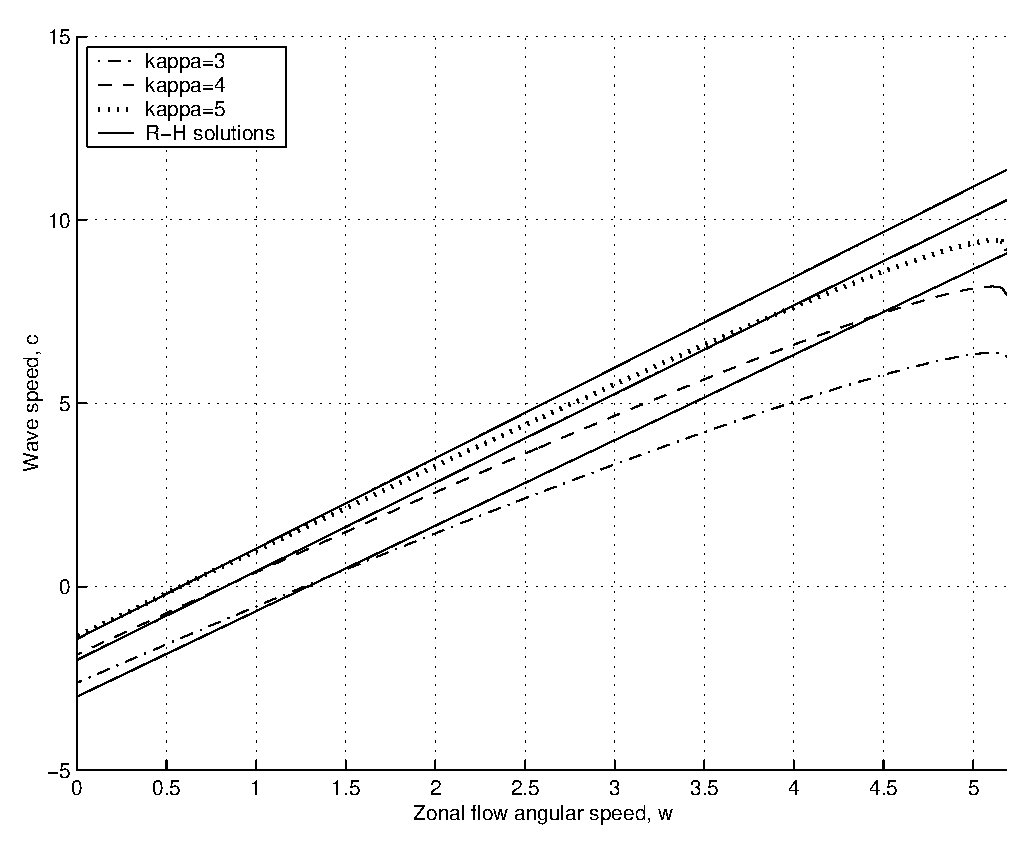
\includegraphics[scale=0.55]{wvchconst1.eps}
	\caption{Comparison of linearized and Rossby--Haurwitz solutions (solid lines) for $\kappa=3,4$ and 5 and $N=100$. The linearized results are shown with dot-dashed, dashed and dotted lines, for $\kappa=3$, 4 and 5 respectively.}
	\label{fig:wvcincomp}
\end{figure}

To compare the two solution types we consider the primary physical eigenvalues for $\kappa=3,4$ and 5 with the equivalent Rossby--Haurwitz solutions over a reasonable range of allowable $\omega$ values. Figure~\ref{fig:wvcincomp} shows the results of this comparison, with the solid lines representing the equivalent Rossby--Haurwitz solution for $\kappa=3$ to 5 from bottom to top respectively. In general one can conclude that the two models are in good broad agreement, especially so for values of $\omega$ in the range $0<\omega<2$ where the effect of the volume matching is minimal.

Note that for $\kappa=3$, 4 and 5 there is a value of $\omega$ for which $c=0$, so that the linearized Rossby wave structure remains stationary relative to the Earth's surface. For values of $\omega$ below this critical value we have wave motion towards the West whereas for values higher we have Eastward wave motion, allowing for a wide variety of atmospheric configurations. Note that the bending over of the linearized solutions for large values of $\omega$ is a consequence of the fact that the height at the poles, $h_o$, is changing to conserve the total volume, as previously discussed.

It is also useful to examine the resulting free surface contours produced by both models. In order to match the height contour levels it it necessary to specify some equivalent value of the wave amplitude $\epsilon$. To make comparison possible we choose to match the two height fields at $(\eta,\phi)=(0,\upi/4)$ which represents a reasonable mid-point level in each contour set. It is interesting to note that despite the fact that Haurwitz did not use a free surface formulation, a resulting equivalent height field may be calculated via an analysis of the pressure field, as developed by \cite{Phillips:NIP}.
\begin{figure}
	\centering
		\includegraphics[scale=0.55]{swfsconts.eps}
	\caption{Linearized free surface contours for $\kappa=4$ with $N=100$.}
	\label{fig:swfsconts}
\end{figure}
\begin{figure}
	\centering
		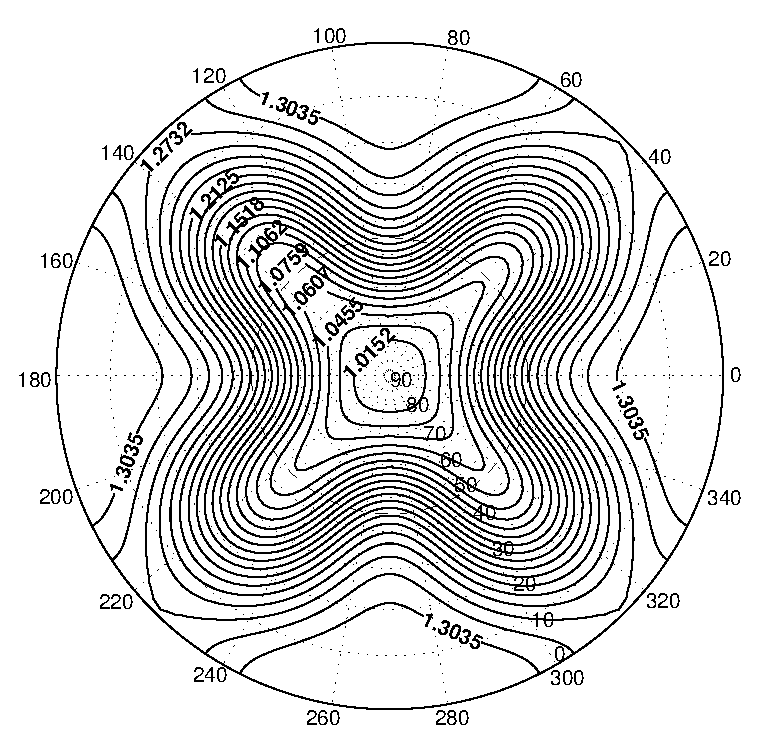
\includegraphics[scale=0.55]{rhfsconts.eps}
	\caption{Rossby--Haurwitz free surface contours for $\kappa=4$.}
	\label{fig:rhfsconts}
\end{figure}

Figures \ref{fig:swfsconts} and \ref{fig:rhfsconts} provide a solution comparison both qualitatively, through a visual comparison, and quantitatively, through the specific contour levels of each height field. The latitudinal circle at $\phi=\upi/4$ is indicated to show where the match takes place. All contour plots were made using a polar sterographic projection of the Northern Hemisphere, described exhaustively by \cite{Snyder:MP}. Of particular interest is the slight pinching of crests and troughs for the Rossby--Haurwitz wave structure that is not evident in the linearized solution. This in turn forces the lower heights, and hence pressures, near the poles to extend further towards the equator in the Rossby--Haurwitz solution. However, overall there is very close agreement between both types of solutions.

\subsection{Nonlinear solution results}
\label{subsec:nonresul}
\subsubsection{Results for $\kappa=4$, $\omega=1.25$}
Figure~\ref{fig:CvsAk4w125} shows wavespeed $c$ computed for $\kappa=4$ and $\omega=1.25$, for each of the three measures of amplitude $\mathcal{A}_{e}$, $\mathcal{A}_{p}$ and $\mathcal{A}_{ave}$ defined previously in \S\,\ref{subsec:ampmeas}. The figure is comprised of a total of 100 separately converged solutions. The truncation levels are $M=20$ and $N=20$ so that each series has a total of 400 coefficients, with a total of 1201 unknowns in the Newton's method algorithm \eqref{eq:updatestep}. Results were initially computed at a lower truncation level of $M=N=10$ to ascertain the general nature of the relationship. Once the nature of the solution was established, $M$ and $N$ were increased.
\begin{figure}
\psfrag{Ap}{\tiny $\mathcal{A}_{p}$}
\psfrag{Ae}{\tiny $\mathcal{A}_{e}$}
\psfrag{Aave}{\tiny $\mathcal{A}_{ave}$}
\psfrag{Wavespeed}{\scriptsize Wavespeed, $c$}
\psfrag{Amplitude}{\scriptsize Amplitude (deg.)}
\psfrag{Linearised}{\tiny Linearized solution}
	\centering
		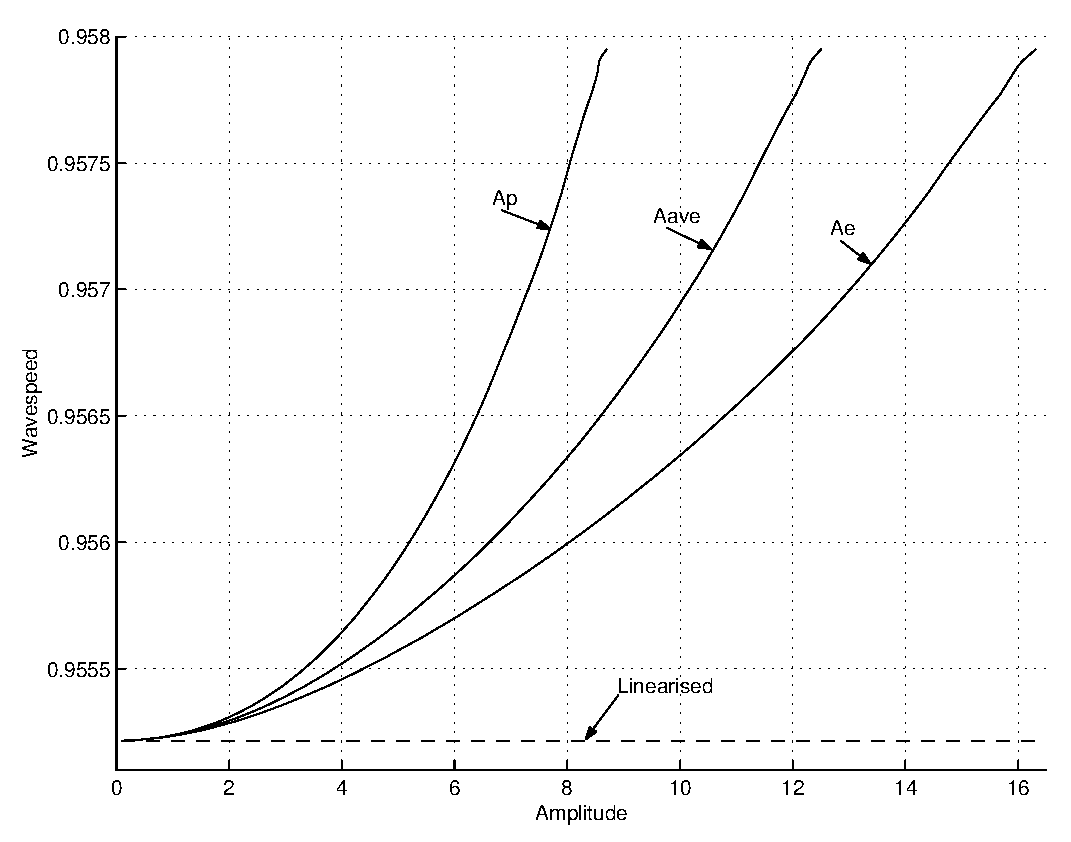
\includegraphics[scale=0.55]{CvsAk4w125.eps}
	\caption{Wavespeed versus amplitude relationship for $\kappa=4$ and $\omega=1.25$}
	\label{fig:CvsAk4w125}
\end{figure}
The error tolerance on the $L^1$ norm of the residual vector was set at $10^{-12}$, leading to average individual residual errors of the order of $10^{-15}$ or less. The agreement between the two levels of representation was found to be excellent, with results at the higher truncation level only differing marginally from those at the lower level, providing evidence for the numerical convergence of the solutions calculated. In particular, bootstrapping was used to increase the truncation level beyond $M=N=20$ for a random sample of points on the solution curve, and in all cases these higher resolution solutions were found to differ negligibly from those for $M=N=20$, and, at least for small amplitude, from those of $M=N=10$ as well.

The linearized solution is included and indicated with a dashed line in figure~\ref{fig:CvsAk4w125}, showing that for small amplitude waves the linear and nonlinear speeds are essentially equivalent. As the amplitude increases the wavespeed also increases, with the curve initially being tangential to the linearized result for small $\mathcal{A}$ but diverging from the linearized result and increasing more rapidly as $\mathcal{A}$ becomes larger. This behaviour is as expected by analogy with other nonlinear wave calculations for gravitationally influenced incompressible fluids, notably those of \cite{Stokes:TOW}, \cite{Schwartz:CEA} and \cite{Cokelet:SGW}. These results, along with contributions from other key researchers in the field, are summarised in the review article by \cite{Schwartz:SNW}.
\begin{figure}
	\centering
		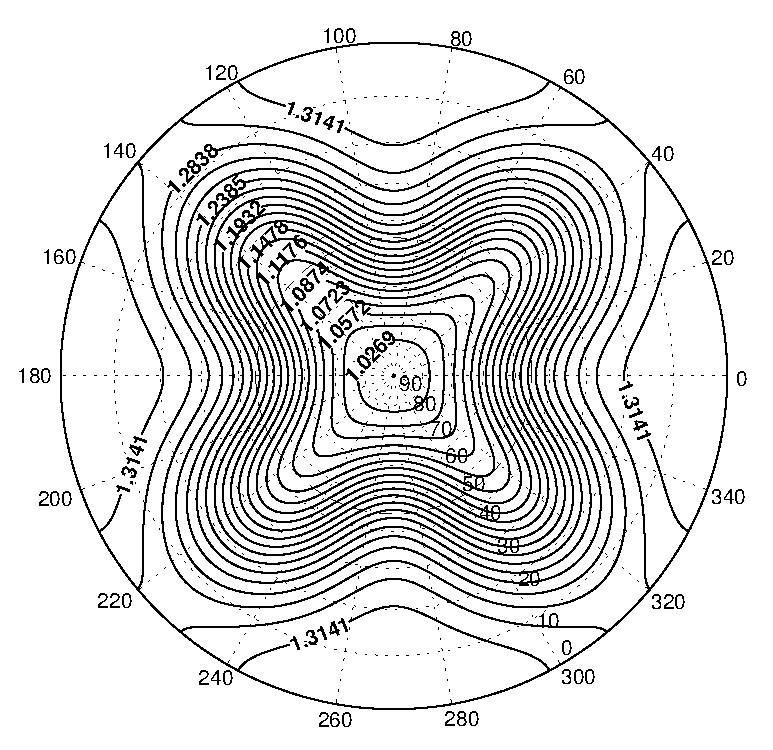
\includegraphics[scale=0.55]{k4w125fsend.eps}
	\caption{Free surface contours at limit of computation for $\kappa=4$, $\omega=1.25$. The average amplitude is $\mathcal{A}_{ave}=12.5104 (deg.)$ and the wavespeed is $c=0.9580$.}
	\label{fig:k4w125fsend}
\end{figure}

As the amplitude continues to increase, the wavespeed increases more rapidly until, ultimately, a limiting case is achieved numerically, where a slight curling over of the curve is observed. The physical explanation of this limiting solution is not clear from this example computation. It is possible, for example, that a sharp crest might be formed somewhere in the flow field, as in the previously mentioned water-wave case studied by Stokes and later by Schwartz. Alternatively, it may be the case that the solution is topologically limited, as found for gravity waves with surface tension by \cite{Schwartz:NSE}, and \cite{Chen:SGC}. However, an analysis of the polar sterographic free surface contours at this limiting wavespeed and amplitude combination, as shown in figure~\ref{fig:k4w125fsend}, suggests that no such behaviour is present. 

We suggest, however, that some type of nonlinear resonance behaviour occurs, which is not accessible to this numerical scheme because of the complexity of the solution space and the  implied sensitivity of Newton's method to the initial guess used. Evidence supporting this statement is presented in the next section. Indeed, it is suspected that the limiting solution indicated in figure~\ref{fig:CvsAk4w125} represents the largest amplitude solution on one particular branch only, and that other solution types may exist with larger amplitudes and wavespeeds. Exhaustive attempts to find such larger waves were made using numerous methods. In particular the algorithm was changed so that the wavespeed became the forcing parameter in an attempt to look for faster progressive waves; however convergence of the residual vector was not obtained. Further analytical work may therefore be necessary to find these extra solution branches.

\subsubsection{Results for $\kappa=4$, $\omega=1.0$}
The solution curves shown in figure~\ref{fig:CvsAk4w1} represent results obtained with the values $\kappa=4$ and $\omega=1.0$; the results consist of 143 separately converged solutions. The truncation levels were set at $M=N=15$ with initial curves mapped out using $M=N=10$; little overall difference was observed between the two resolutions. The error tolerance on the $L^1$ norm of the residual vector was set at $10^{-12}$, leading to average individual residual errors of the order of $10^{-15}$ or less. Like the previous example, the solution agrees well with the linearized result for small amplitude waves and as $\mathcal{A}$ increases so does the wavespeed $c$. However, as opposed to the previous case for $\omega=1.25$, distinct discontinuous jumps are now evident, dividing the solution curves into separate branches, between which no numerical solutions were able to be computed to adequate convergence. The individual branches have been labelled in the figure and will be refered to subsequently as branches 1 through 5 respectively.

Discrete branching of the solution, as evidenced in the present results, is characteristic of nonlinear resonance interaction in general, in which certain energy states of the system can be viewed as sympathetically exciting the underlying wave motion, undergoing energy exchange between waves of different wavelengths in the process. Nonlinear resonance has been known to exist in complex nonlinear wave propagation problems for some time now. In the context of gravity waves with surface tension \cite{Wilton:OR} encountered key values of the capillary number at which resonance occured. \cite{Schwartz:NSE}, and \cite{Hogan:SES1,Hogan:SES2,Hogan:SES3}, confirmed this behaviour in detail, by numerically solving the exact equations, and found that multiple simultaneous solution branches were possible. \cite{Forbes:SWL1,Forbes:SWL2} also found resonant behaviour for surface waves of large amplitude beneath an elastic sheet. 
\begin{figure}
\psfrag{Ap}{\tiny $\mathcal{A}_{p}$}
\psfrag{Ae}{\tiny $\mathcal{A}_{e}$}
\psfrag{Aave}{\tiny $\mathcal{A}_{ave}$}
\psfrag{Wavespeed}{\scriptsize Wavespeed, $c$}
\psfrag{Amplitude}{\scriptsize Amplitude (deg.)}
\psfrag{Linearised}{\tiny Linearized solution}
\psfrag{B1}{\tiny Branch 1}
\psfrag{B2}{\tiny Branch 2}
\psfrag{B3}{\tiny Branch 3}
\psfrag{B4}{\tiny Branch 4}
\psfrag{B5}{\tiny Branch 5}
	\centering
		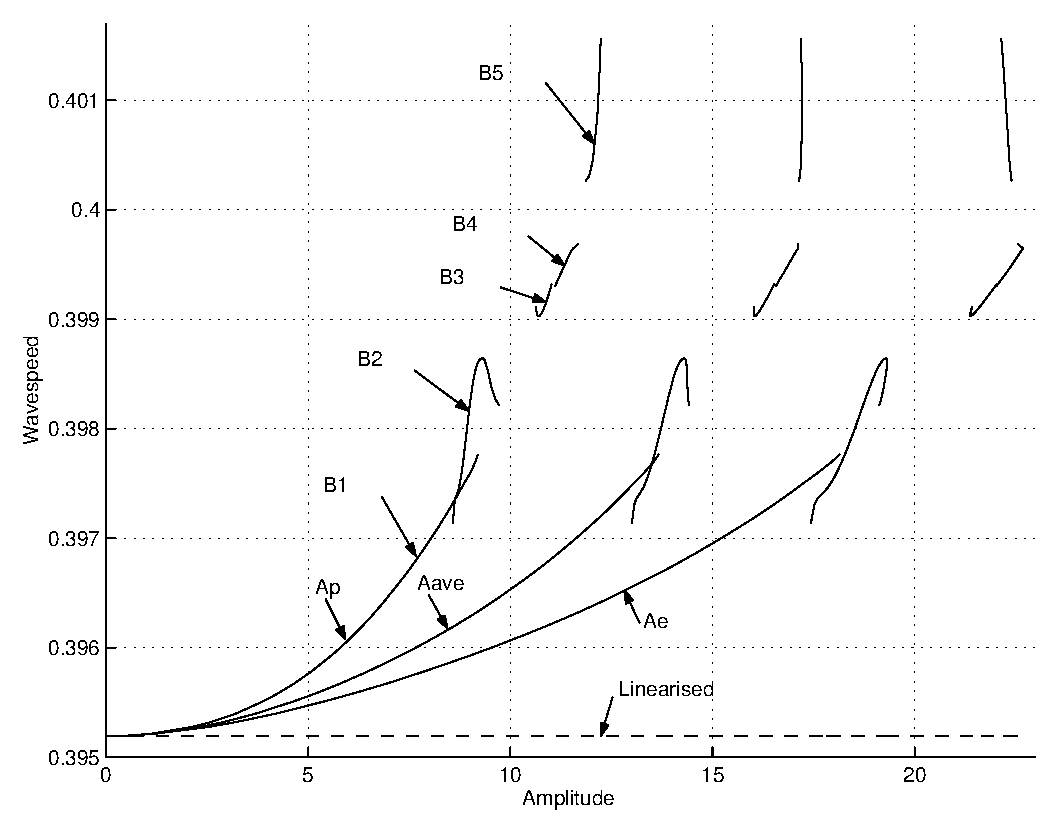
\includegraphics[scale=0.55]{CvsAk4w1.eps}
	\caption{Wavespeed versus amplitude relationship for $\kappa=4$ and $\omega=1.0$}
	\label{fig:CvsAk4w1}
\end{figure}

In the meteorological context, \cite{Longuet:RIP} showed that resonant interactions over time can exist between three waves, termed a resonant triad, obeying certain algebraic relationships relating the individual wavenumbers and corresponding wavespeeds; their results are concerned with planetary waves both on the $\beta$-plane and more generally on a spherical surface. Both \cite{Hoskins:SRH} and \cite{Baines:SPW} extend this work by considering the stability of planetary waves and calculating amplitudes required for instability based on triad interactions for specific types of Rossby--Haurwitz waves.

To understand how the resonance is occuring in this particular example we can view the system as being forced by the parametrized amplitude through the Fourier coefficient $H_{1,1}$. As $H_{1,1}$ increases, $\mathcal{A}$ and $c$ also increase until a point is reached where some of the Fourier modes in the series expansions are naturally excited  by the forcing and can absorb energy via nonlinear interactions. At this point resonance occurs and the system becomes unstable in the sense that unchanging progressive waves are no longer possible. We can thus think of resonance in this instance as a parameter region of, possibly highly oscillatory, transition between two separate progressive-wave states for the full nonlinear time dependent problem. The fundamental nature of any resonance demands that the amplitude of the dominant harmonic wave grow in time. As we are only concerned with progressive waves this type of behaviour is excluded at the outset when we defined our traveling coordinate transform \eqref{eq:etadef}. However, as indicated by the results, the method used is still able to expose fundamental resonances of the system where full time dependence would be necessary to discern the complete behaviour of the dynamical system.
\begin{figure}
	\centering
		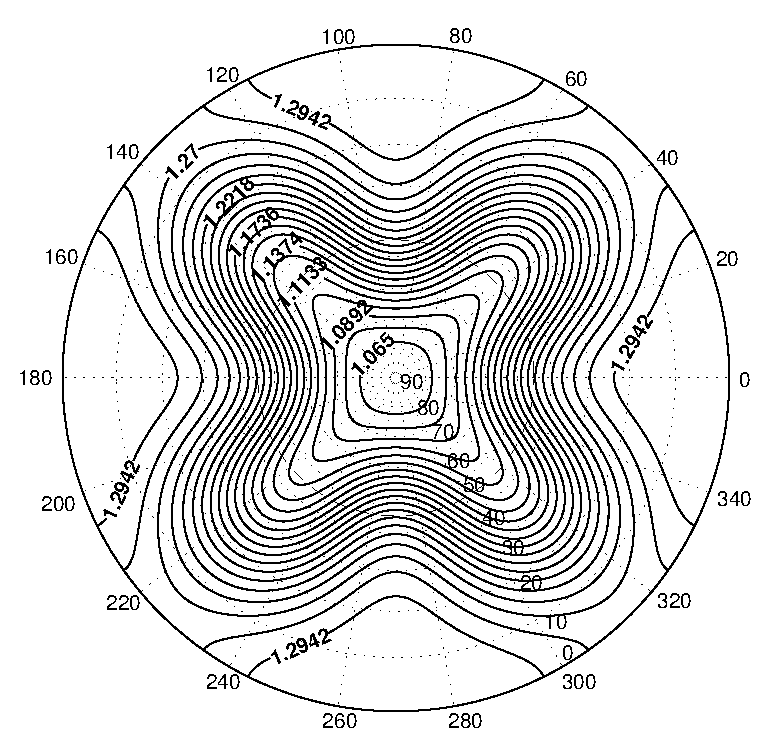
\includegraphics[scale=0.55]{k4w1fsb1end.eps}
	\caption{Free surface contours at end of branch 1 for $\kappa=4$, $\omega=1.0$. The average amplitude is $\mathcal{A}_{ave}=13.6732 (deg.)$ and the wavespeed is $c=0.3978$.}
	\label{fig:k4w1fsb1end}
\end{figure}

The separate branches of the solution curve shown in figure~\ref{fig:CvsAk4w1} can be classified, at least partially, in terms of the general associated height field structure and corresponding velocity vector field along each solution curve segment. On branch 1 we conclude that at no point in the flow does the fluid move counter to the general direction of the overall wave propagation direction and additionally that the only stagnation points in the flow field are located at either of the two topological poles, as expected. The free surface contours at the limiting upper value of branch 1 are shown in figure~\ref{fig:k4w1fsb1end}. It is observed that the general character of these contours is quite similar to those obtained with both the linearized model and Rossby--Haurwitz theory.

For solutions along branch 2, not much difference was observed between those along branch 1, with the general flow properties of the previous paragraph applying equally well here. It is also important to emphasize that the apparent intersection of branches 1 and 2 in the diagram is not a bifurcation point. Examination of the Fourier coefficients in the neighbourhood of the overlap shows distinctly different solution structure for each branch which fail to converge to a common set, despite the fact that the values of $\mathcal{A}$ and $c$ for the two branches coincide at this point. It would be possible to prove this with a simple analysis of the determinant of the Jacobian near the point of apparent intersection, as in \cite{Chen:NEE}; however the ease with which the Newton method iterates through this region seems to suggest that no further investigation is necessary with regard to the possible existence of a bifurcation. Additionally, the solution curve for the equatorial amplitude $\mathcal{A}_{e}$ does not contain the intersection, which confirms the presence of a resonance, instead of a simple bifurcation.

Solutions on branches 3 and above reveal richer dynamics in terms of more stagnation points in the flow field, reverse flow leading to localized circulation, and highly nonlinear wave profiles. The main difference between the lower solution branches 1 and 2 and the upper solution branches 3, 4 and 5 can be expressed by examining the number of stagnation points in the flow field, disregarding the obvious polar stagnation points that all solutions must have by definition of the series expansions themselves. It is evident that for solutions on branches 3 and higher, all have stagnation points located symmetrically on the equator about the coordinate lines $\eta=2n\upi/\kappa$, for $n=0,1,\ldots,\kappa-1$. The exact position of these stagnation points was noted to change as the amplitude varied, although typically they were located quite close to the symmetry lines themselves. In between the two stagnation points the fluid was observed to flow counter to the general direction of the progressive wave movement. The height field was examined for small-scale localized high-pressure cells at these points of circulation, but none were found.

Figure~\ref{fig:k4w1fsb4end} shows a typical free surface contour plot for solutions along branches 3 and 4. The figure actually shows the contours at the limiting upper value of branch 4 and so represents the maximum allowable amplitude for waves on branch 4. It seems, from an analysis of the velocity fields and height contours, that the qualitative difference between waves on branches 3 and 4 is negligible. Nonetheless, a distinct gap was encountered when trying to establish the continuity of the solution between branches 3 and 4. Further investigation is needed to establish the key qualitative differences between these two branches, although this is both beyond the scope and computational capability of the present work.

Of particular note is the way in which low-level polar heights, and hence pressures, are seen to move equator-ward for solutions along these branches. It is suspected that the limiting factor for wavespeeds and amplitudes towards the upper end of branch 4 is directly related to the topology of the low-level free surface contours which are not able to bend inwards any further without creating an isolated cut-off low-pressure system in the flow field. This statement is supported by the following analysis of branch 5 solutions.
\begin{figure}
	\centering
		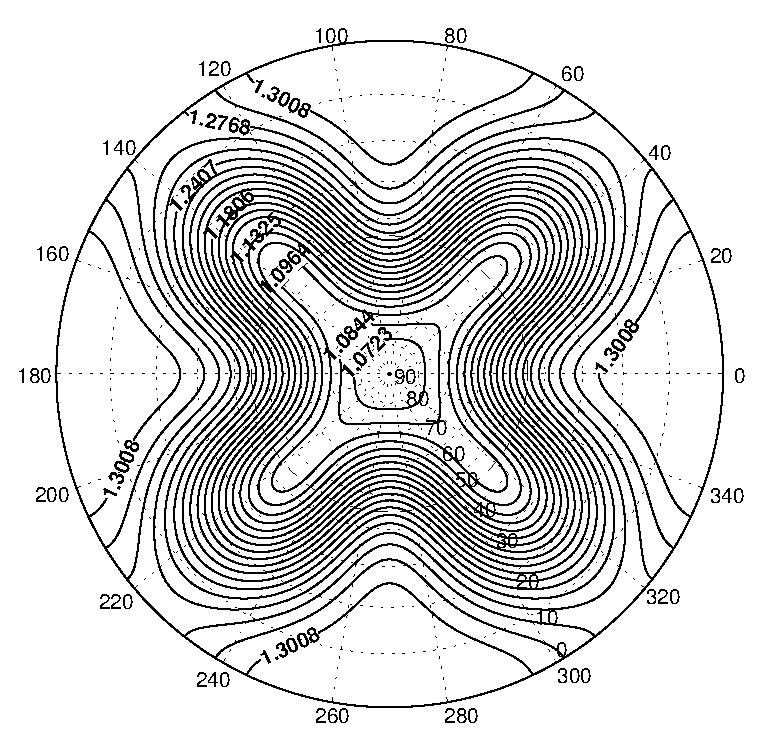
\includegraphics[scale=0.55]{k4w1fsb4end.eps}
	\caption{Free surface contours at end of branch 4 for $\kappa=4$, $\omega=1.0$. The average amplitude is $\mathcal{A}_{ave}=17.11662 (deg.)$ and the wavespeed is $c=0.3997$.}
	\label{fig:k4w1fsb4end}
\end{figure}

The highly nonlinear free surface height contours for the upper end of branch 5 are shown in figure~\ref{fig:k4w1fsb5end}. It is immediately evident that solutions along this branch have the distinguishing feature of cut-off low-pressure cells which are isolated from the general progressive wave structure. In addition to the already mentioned stagnation points in the flow field for waves on branches 3 and higher, more stagnation points are introduced for waves on the fifth branch, this time occuring close to the poles of the coordinate system rather than on the equator. It was initially suspected that the centre of each cut-off low-pressure cell must be a stagnation point; however careful analysis of the velocity vector field did not confirm this. Nonetheless the velocity in the vicinity of these cells is quite small compared to the rest of the flow field and can be described as circulatory about the centre of each cell.
\begin{figure}
	\centering
		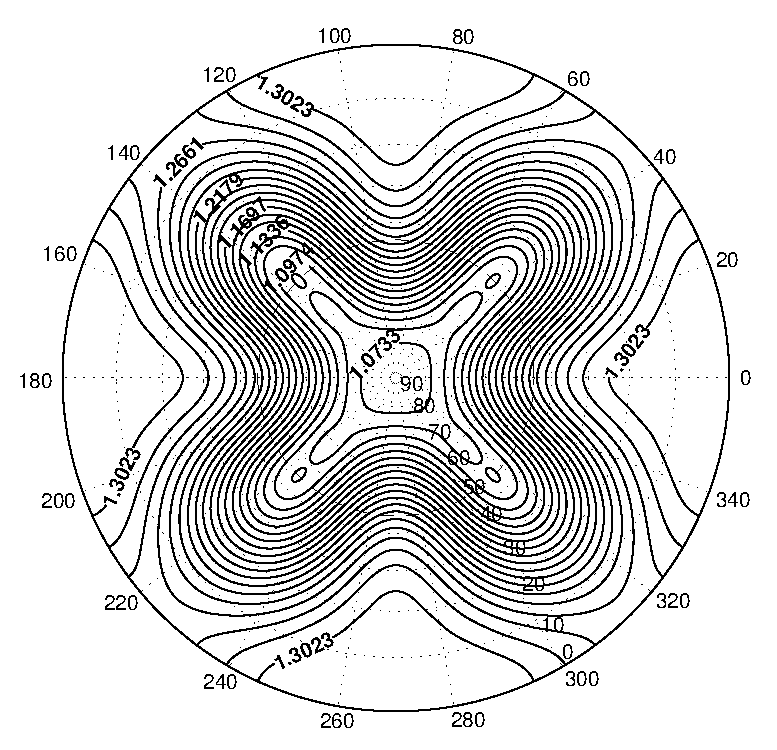
\includegraphics[scale=0.55]{k4w1fsb5end.eps}
	\caption{Free surface contours at end of branch 5 for $\kappa=4$, $\omega=1.0$. The average amplitude is $\mathcal{A}_{ave}=17.11662 (deg.)$ and the wavespeed is $c=0.4016$.}
	\label{fig:k4w1fsb5end}
\end{figure}

It is of interest to note that the stagnation points introduced for branch 5 solutions occur immediately below each cut-off low-pressure cell as indicated in figure~\ref{fig:k4w1fsvvb5end}. Also shown are all previously mentioned stagnation points as well as regions of circulation, labeled reverse flow. We can conclude that generally the flow is seen to be geostrophic in the sense that the streamlines are nearly parallel to the isobars. This is clearly true in the neighbourhood of the perturbed $\phi=\pm\upi/4$ zonal flow contour that forms the basis of the numerical analysis in this section.
\begin{figure}
\psfrag{Stagnation points}{\scriptsize Stagnation points}
\psfrag{Reverse Flow}{\scriptsize Reverse flow}
	\centering
		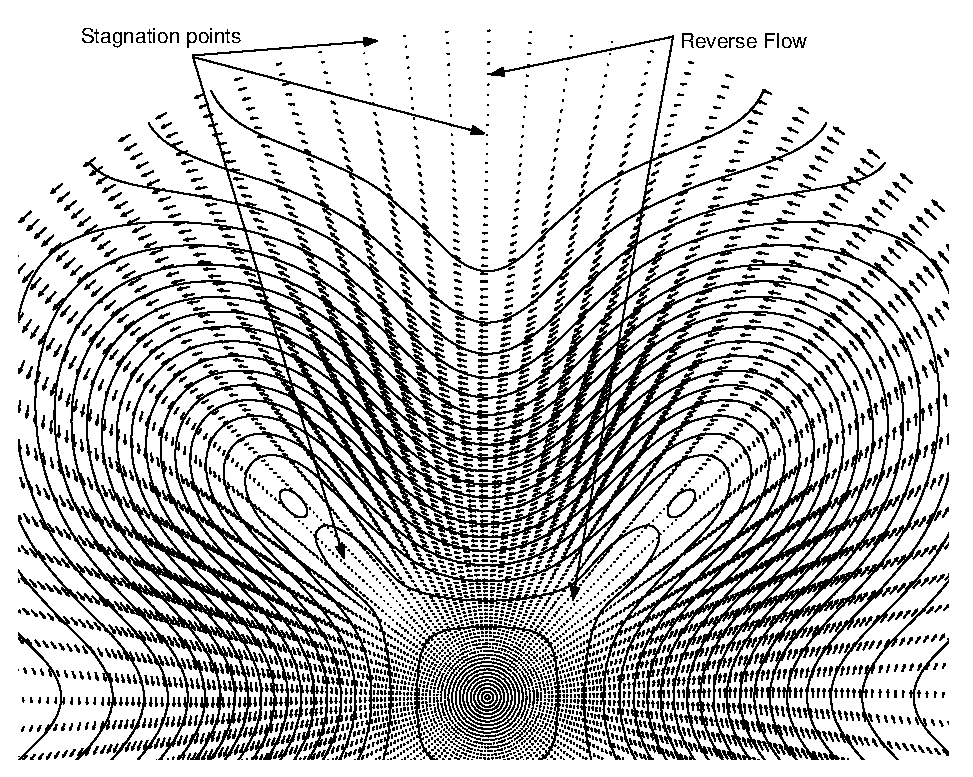
\includegraphics[scale=0.55]{k4w1fsvvb5end.eps}
	\caption{Free surface contours with corresponding velocity vector field at end of branch 5 for $\kappa=4$, $\omega=1.0$. The average amplitude is $\mathcal{A}_{ave}=17.11662 (deg.)$ and the wavespeed is $c=0.4016$.}
	\label{fig:k4w1fsvvb5end}
\end{figure}

The fate of the solution curves past the end of branch 5 is still uncertain. Attempts were made to compute more points beyond the limits shown but in all cases convergence was not achieved. It might be that our numerical method is not well suited to computing past points where the slope of the curve is nearly infinite, in which case improved techniques are required to investigate the behaviour past the limit shown. Alternatively this may be close to the maximum allowable amplitude of the system, imposed as a consequence of the finite size and topology of the sphere. An analysis of the constraints of potential vorticity conservation of Rossby waves on a $\beta$-plane by \cite{Lindzen:NLR} revealed that there are finite limits to the size of Rossby wave amplitudes. This reasoning should apply even more so to the sphere where the finite size becomes an important attribute of the problem.

\subsubsection{Results for $\kappa=5$, $\omega=1.25$}
It is of interest to study how the dynamical system behaves with an alternative value of the wave number $\kappa$. We now present results obtained with $\kappa=5$, using the same pair of values ($\omega=1.25$ and $\omega=1.0$) for the dimensionless zonal flow super rotation; in this section we examine the case $\omega=1.25$. Figure~\ref{fig:CvsAk5w125} shows the computed wave-speed versus amplitude relationship using a truncation of $M=N=20$ for 203 individually converged solutions. The error tolerance on the $L^1$ norm of the residual vector was set at $10^{-12}$, leading to average individual residual errors of the order of $10^{-15}$ or less.
\begin{figure}
\psfrag{Ap}{\tiny $\mathcal{A}_{p}$}
\psfrag{Ae}{\tiny $\mathcal{A}_{e}$}
\psfrag{Aave}{\tiny $\mathcal{A}_{ave}$}
\psfrag{Wavespeed}{\scriptsize Wavespeed, $c$}
\psfrag{Amplitude}{\scriptsize Amplitude (deg.)}
\psfrag{Linearised}{\tiny Linearized solution}
\psfrag{B1}{\tiny Branch 1}
\psfrag{B2}{\tiny Branch 2}
	\centering
		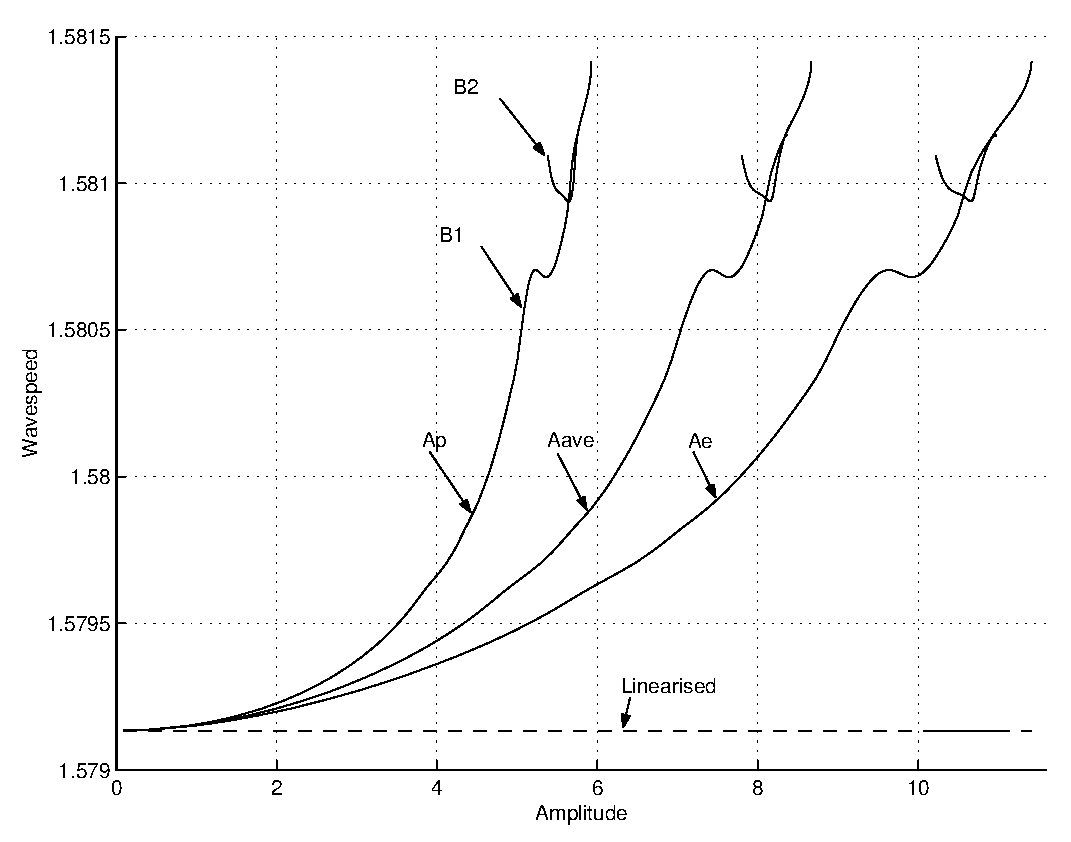
\includegraphics[scale=0.55]{CvsAk5w125.eps}
	\caption{Wavespeed versus amplitude for $\kappa=5$ and $\omega=1.25$}
	\label{fig:CvsAk5w125}
\end{figure}

The same general trend as for $\kappa=4$ is encountered here for $\kappa=5$, with the linearized solution being a good approximation to the nonlinear solution for small $\mathcal{A}$ and the wavespeed becoming increasingly greater as the amplitude is increased. It appears that the use of $\kappa=5$ introduces a new phenomenon in the form of a localized cubic structure located near $c\approx1.5807$. It was initially suspected that this was in fact two distinct branches separated by a resonance; however it was possible to compute continuously through this region, using a very small step size, without encountering any non convergent solutions. 

Therefore it seems that there are at least two explanations for this behaviour. The first is that there is in fact a resonance occuring near the point of inflexion, but existing on such a small scale that we were unable to detect in on any occasion. This does not seem very likely given the nature of the previous nonlinear resonances observed for the case $\kappa=4$, $\omega=1.0$. The second explanation is that this is a feature of the dynamics and forcing, in which energy exchange between certain wavelengths is taking place in such a maner as to increase the overall amplitude while at the same time reducing the wave-speed. If so, this would represent a type of damped resonance, but careful analytical work, beyond the scope of this study, would be needed to identify the physical nature of the damping mechanism. Despite this localized reversal of the general trend of the graph, no obvious distinguishing features are visible when we examine the free surface contours and velocity vector field in the vicinity of this solution region. This fact seems to support the conjecture that separate resonance branches do not exist in this case.

Two separate solution branches were found to exist towards the upper end of the curve when the limiting wavespeed-amplitude combination was approached. Because it is not entirely clear from the figure, it needs to be emphasized that the first branch terminates in the vicinity of $c\approx1.5812$; thus the highest possible wavespeed indicated is at the right end of branch 2. It is again unlikely that the apparent intersection of the two branches is a sign of a simple bifurcation, for reasons outlined in the previous section.

For the left end of the second branch, numerical results have in fact been computed well beyond the termination point shown in the figure. However, it appears that they are of questionable value due to increasing numerical error along that branch and have therefore not been shown. The ultimate fate of this upper branch is not clear and may perhaps require alternative numerical techniques to reveal. In any event it is possible that this branch is physically unstable, the system preferring the lower wavespeed over the higher one, and so would generally not be observed in practice. It is even possible that a physical instability in this branch might produce a numerical instability, since the numerical iteration process may be equivalent to stepping forward in time \cite*[see][page 149]{Ames:NMP}.

Typical free surface contours of the system are presented in figure~\ref{fig:k5w125fsb1end}, showing the nature of the solution at the end of branch 1. In contrast to the highly nonlinear structures computed at the end of the curve for $\kappa=4$ and $\omega=1.0$, these contours exemplify the significantly smaller maximum amplitude for which a convergent wavespeed was able to be calculated. In addition, no defining qualitative features of the velocity field were found that could be used to distinguish easily between the two solution branches. It is possible that more solution curves exist beyond those that are indicated; however attempts to find such solutions were not successful. 
\begin{figure}
	\centering
		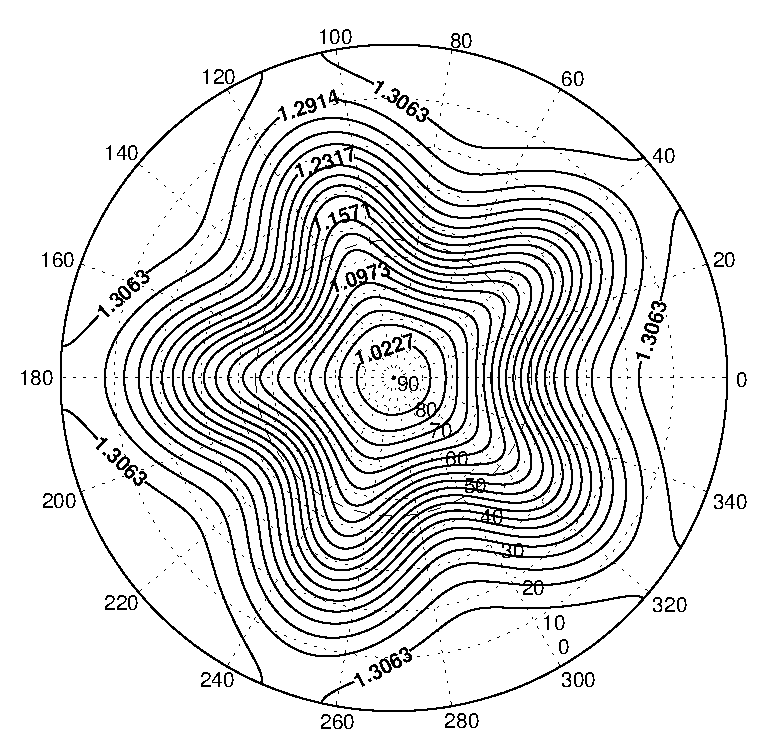
\includegraphics[scale=0.55]{k5w125fsb1end.eps}
	\caption{Free surface contours at end of branch 1 for $\kappa=5$, $\omega=1.25$. The average amplitude is $\mathcal{A}_{ave}=8.3678 (deg.)$ and the wavespeed is $c=1.5812$.}
	\label{fig:k5w125fsb1end}
\end{figure}

\subsubsection{Results for $\kappa=5$, $\omega=1.0$}
For completeness we present results in this final section for $\kappa=5$ and $\omega=1.0$. Figure~\ref{fig:CvsAk5w1} shows the computed solution curves obtained with the truncation level $M=N=15$ for 100 individually converged solutions. The error tolerance on the $L^1$ norm of the residual vector was again set at $10^{-12}$. The general features of this figure are less remarkable than those for the preceding set of results obtained with $\omega=1.25$, although there is some evidence for a similar localized cubic structure, this time in the vicinity of $c=0.99395$. The severity of this local cubic behaviour, however, is significantly less noticeable and does not substantially influence the general increase of $c$ with $\mathcal{A}$. As in all previous solution curves presented, the results here agree well with the linearized value of the wavespeed for small values of the amplitude.
\begin{figure}
\psfrag{Ap}{\tiny $\mathcal{A}_{p}$}
\psfrag{Ae}{\tiny $\mathcal{A}_{e}$}
\psfrag{Aave}{\tiny $\mathcal{A}_{ave}$}
\psfrag{Wavespeed}{\scriptsize Wavespeed, $c$}
\psfrag{Amplitude}{\scriptsize Amplitude (deg.)}
\psfrag{Linearised}{\tiny Linearized solution}
	\centering
		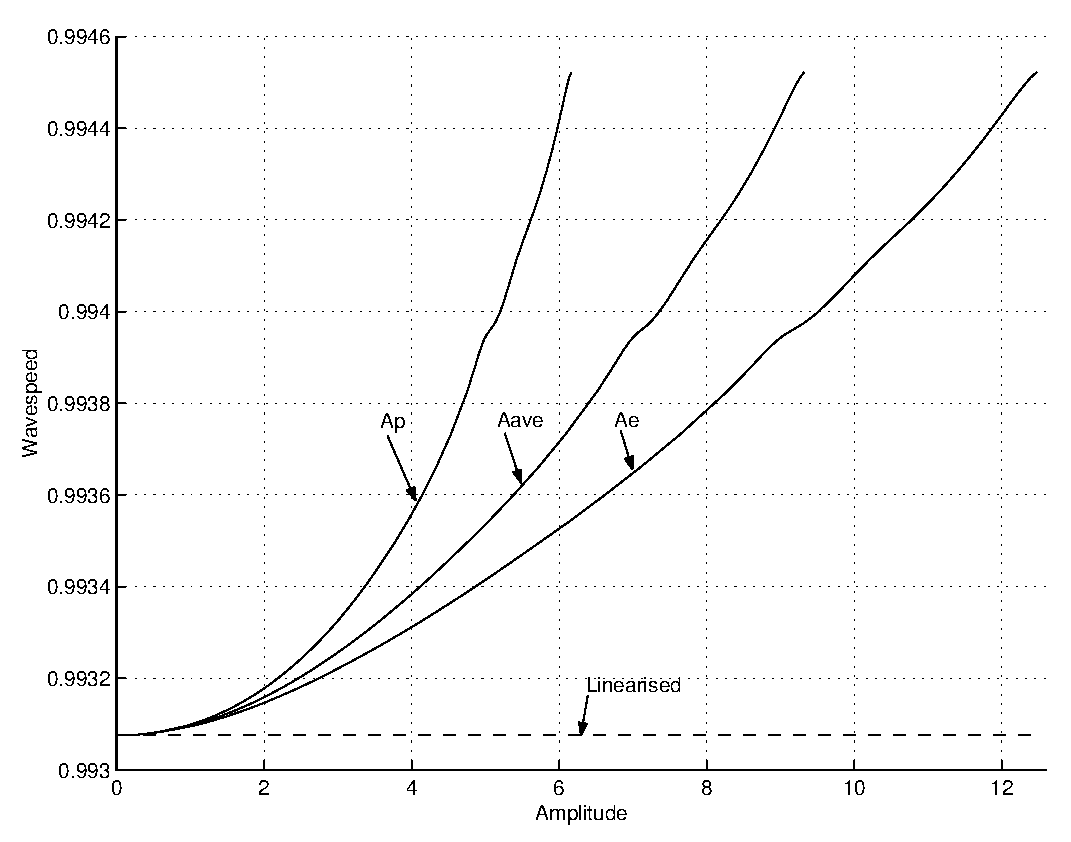
\includegraphics[scale=0.55]{CvsAk5w1.eps}
	\caption{Wavespeed versus amplitude for $\kappa=5$ and $\omega=1.0$}
	\label{fig:CvsAk5w1}
\end{figure}

Typical free surface contours at the right end of the one and only computed branch are shown in figure~\ref{fig:k5w1fsend}. The waves shown are in general highly nonlinear and it should be noted that the maximum possible amplitude obtained with this slower zonal super rotation speed is larger than that obtained with $\omega=1.25$. No additional stagnation points in the flow field were observed, as in the previous case, and consequently all fluid flow was found to be in the same direction as the direction of propagation of the progressive wave. 

It is again suspected that there are in fact more solution branches in addition to the one shown in figure~\ref{fig:CvsAk5w1}. To support this statement we argue that the general nature of the flow field at the limiting computed value seems to be rather well behaved with no clearly identifiable limiting topological features. Unsuccessful attempts were made to bootstrap the limiting solutions to those on another higher branch; in all cases adequate convergence of the residual vector was not achieved. 

\begin{figure}
	\centering
		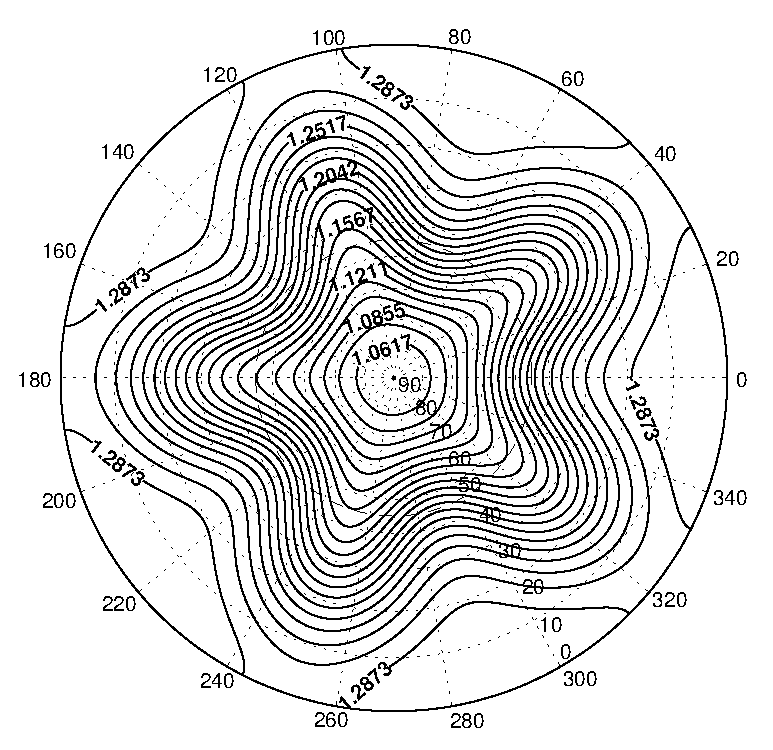
\includegraphics[scale=0.55]{k5w1fsend.eps}
	\caption{Free surface contours at end of branch 1 for $\kappa=5$, $\omega=1.0$. The average amplitude is $\mathcal{A}_{ave}=9.3175 (deg.)$ and the wavespeed is $c=0.9945$.}
	\label{fig:k5w1fsend}
\end{figure}

\section{Discussion and Conclusion}
\label{sec:conclus}
In this paper we have presented a detailed picture of how the effects of nonlinearity influence the relationship existing between wavespeed and amplitude for progressive Rossby waves. The techniques utilised have uncovered feature-rich dynamical properties of progressive-wave solutions of the incompressible shallow atmosphere equations on a rotating sphere. In particular it was shown that nonlinear resonance plays an important and dominant role for waves with large amplitudes. The effect of resonance was observed to separate solutions of the system into disjoint regions, with similar solutions lying on the same solution branch in wavespeed--amplitude space.

For slowly propagating progressive waves with longitudinal wavenumber $\kappa=4$ and zonal flow angular speed $\omega=1.0$, it was shown that if the amplitude forcing becomes large enough it is possible for the flow to develop localized low-pressure cells in the mid-latitude regions. These types of extreme amplitude solutions were accompanied by stagnation points in the flow field at locations other than the poles. In general it was observed that for these highly nonlinear waveforms the lower polar free-surface heights, and hence pressures, and also the higher equatorial free-surface elevations, tended to be grossly distorted so that it was common for contours originating near the equator or pole to be deformed towards regions well in excess of the mid-latitudes.

The linearized wavespeed associated with this specific parameter configuration was $c\approx 0.395$. Thus for only a slightly smaller value of the zonal flow parameter $\omega$, the linearized and associated nonlinear wavespeeds would be very close to zero, so that the Rossby wave would be approximately stationary with respect to the the surface of the Earth. We conjecture that the particular nature of the wavespeed--amplitude relationship for stationary Rossby waves would not be dissimilar to that computed for the case $\kappa=4$ and $\omega=1.0$. If this is so it would imply the existence of highly distorted nearly stationary Rossby waves containing high pressure ridges extending polewards from the equator, with cut-off low pressure cells in the mid-latitudes. This type of atmospheric configuration could be seen as being crucial to the instigation of an atmospheric blocking event, with subsequent development of cut-off high-pressure cells near the mid-latitudes when full time dependence is included in the model. 

This argument is, in general, supported by the work of \cite{Austin:BML}, who found that the splitting of westerly winds by blocking is attributable to interference, or resonance, between planetary waves with very large amplitudes. In this conjecture, however, nothing is implied as to how the dynamical system moves from one solution branch to the next. Nor is it expected that all the solution branches would be physically stable. However, it is possible that through various forcing mechanisms, such as the effects of topography and thermal heating/cooling, the atmosphere can pass from one equilibrium state to another. If this proves to be true then the highly nonlinear feature-rich solutions calculated in this work would support the idea that blocking is primarily a dynamical state which is accessible through appropriate forcing of the atmospheric system.

\begin{acknowledgments}
T.\,G.\,C. gratefully acknowledges the provision of an APA (Australian Postgraduate Award) which has enabled him the time to conduct this research as part of a PhD degree. 
\end{acknowledgments}

\bibliography{rossby}
\bibliographystyle{jfm}

\end{document}
